\documentclass[11pt]{article}
\usepackage[margin=1in]{geometry}
\usepackage{amsmath}
\usepackage{booktabs}
\usepackage{graphicx}
\usepackage{subcaption}
\usepackage[hidelinks]{hyperref}
\usepackage[T1]{fontenc}
\usepackage{lmodern}
\usepackage{microtype}
\usepackage[section,above,below]{placeins}
\renewcommand{\topfraction}{0.9}
\renewcommand{\bottomfraction}{0.5}
\renewcommand{\textfraction}{0.07}
\renewcommand{\floatpagefraction}{0.8}

\title{FastSAR: High-Throughput, High-Fidelity Open-Source SAR Image Formation on CPUs, GPUs and TPUs}
\author{Paul Singerman\\ Penn State University\\ \texttt{pgs16@psu.edu} \and Tom Braun\\ Penn State University\\ \texttt{trb5864@psu.edu}}
\date{October 2026}

\setlength{\belowcaptionskip}{5pt}

\begin{document}
\maketitle

\begin{abstract}
Exact backprojection of a spaceborne SAR collection needs one interpolated read per pixel and pulse, @@sc.panama.lookups@@~trillion for a 12,207 by 8,808~pixel Umbra image of the Panama Canal. ISCE3, the fastest of the open-source backprojections evaluated here that produce an image of this collection, would take an estimated 4.8~h on a 16-vCPU instance. FastSAR is an open-source library with backprojection kernels for CPUs, NVIDIA GPUs and Google TPUs. Its factorized backprojection forms the image in @@t.panama.cpu-c4d16.ffbp.fp32_cpp.s@@~s on that instance, @@t.panama.gpu-l4.ffbp.fp32_cuda.s@@~s on an NVIDIA L4, and @@t.panama.tpu-v5e.ffbp.fp32_high_pallas2_direct.s@@ and @@t.panama.tpu-v6e.ffbp.fp32_high_pallas2_direct.s@@~s on Google TPU v5e and v6e. The errors of its float32 and float16 images in three regions are @@truth.abs.worst@@ to @@truth.abs.best@@~dB relative to a float64 exact backprojection. Its own exact backprojection, @@exact.l4.dur@@ on the L4, is @@truth.margin.lo@@ to @@truth.margin.hi@@~dB more accurate than its float32 image. At float32 accuracy (three-pass bfloat16 products on the TPUs) a thousand images cost \$@@c.panama.l4.fp32.usd@@ on the L4, \$@@c.panama.v5e.high.usd@@ to \$@@c.panama.v6e.high.usd@@ on the TPUs and \$@@c.panama.cpu-c4d16.ffbp.fp32_cpp.usd@@ on the CPU. On five Capella collections, including a sliding spotlight and two stripmaps, FastSAR's worst-region error is @@modes.err.worst@@ to @@modes.err.best@@~dB, @@modes.isce3.cphd.margin.min@@ to @@modes.isce3.cphd.margin.max@@~dB below ISCE3's when both are scored with the per-pulse antenna positions of the phase-history files.
\end{abstract}

\section{Introduction}

Image formation turns a SAR phase history of $10^8$ to $10^9$ complex samples into an image with a comparable number of pixels (Table~\ref{tab:scenes}). Exact backprojection makes no approximation to the imaging geometry~\cite{jakowatz1996,gorham2010}, and its cost scales with the product of the pixel and pulse counts; for the Panama collection of Table~\ref{tab:scenes} that product is @@sc.panama.lookups@@~trillion interpolated reads. The three open-source backprojections that produce an image of this collection, RITSAR, the Air Force Research Laboratory (AFRL) toolbox and ISCE3, would take an estimated 4.8 to 69~h on a 16-vCPU instance (Table~\ref{tab:oss}).

FastSAR is an open-source SAR image formation library with one Python interface for CPUs, NVIDIA GPUs and Google TPUs (Section~\ref{sec:fastsar}). On the Panama collection it forms a float32-class image (float32 arithmetic or its TPU equivalent, Section~\ref{sec:protocol}) @@oss.isce3.cpu.ratio@@ times faster than ISCE3's estimate on the same CPU instance and @@oss.isce3.l4.ratio@@ times faster on an NVIDIA L4 (Table~\ref{tab:oss}).

Its error in the lock, port and ship regions is 3.9 to 6.7~dB below the lowest open-source error, that of the AFRL toolbox's \texttt{bpBasic}, and about 25 to 30~dB below ISCE3's off-center patches (Section~\ref{sec:oss}). The other open-source backprojections are slower still, by estimated factors of up to @@oss.ratio.max@@ (Table~\ref{tab:oss}). A thousand images cost \$@@c.panama.l4.fp32.usd@@ on the L4 (Table~\ref{tab:cost}). FastSAR's exact backprojection, which has separate CPU and CUDA kernels, lowers the error by a further @@truth.margin.lo@@ to @@truth.margin.hi@@~dB (Section~\ref{sec:quality}) at @@exact.vs.ffbp.cpu@@ times the factorized time on the CPU and @@exact.time.l4.panama@@ times on the L4 (Table~\ref{tab:cost}).

The factorized algorithm is written as tile-wise phase rotations and decimation filters followed by dense matrix products, with a kernel for each device (Section~\ref{sec:fastsar}). In the profiled builds each stage runs within 1.0 to 2.5 times a lower bound set by the hardware unit that limits it (Table~\ref{tab:bounds}, Appendix~\ref{app:kernels}).

Of the four devices evaluated (two TPU generations, one GPU and one CPU instance, Table~\ref{tab:platforms}), the L4 forms the float32-class image at the lowest cost (Table~\ref{tab:cost}). Reduced precision, float16 throughout on the L4 and single-pass products on the TPUs, lowers the cost by @@l4.f16.saving.pct@@\% and by @@sp.saving.v6e.pct@@ to @@sp.saving.v5e.pct@@\% and raises the error by @@l4.f16.loss@@ and @@sp.vs.3pass.db@@~dB (Sections~\ref{sec:quality} and~\ref{sec:cost}). On five Capella collections in three modes the float32-class errors stay below $-59$~dB (Table~\ref{tab:modes}).

\begin{figure}[tbp]
\centering
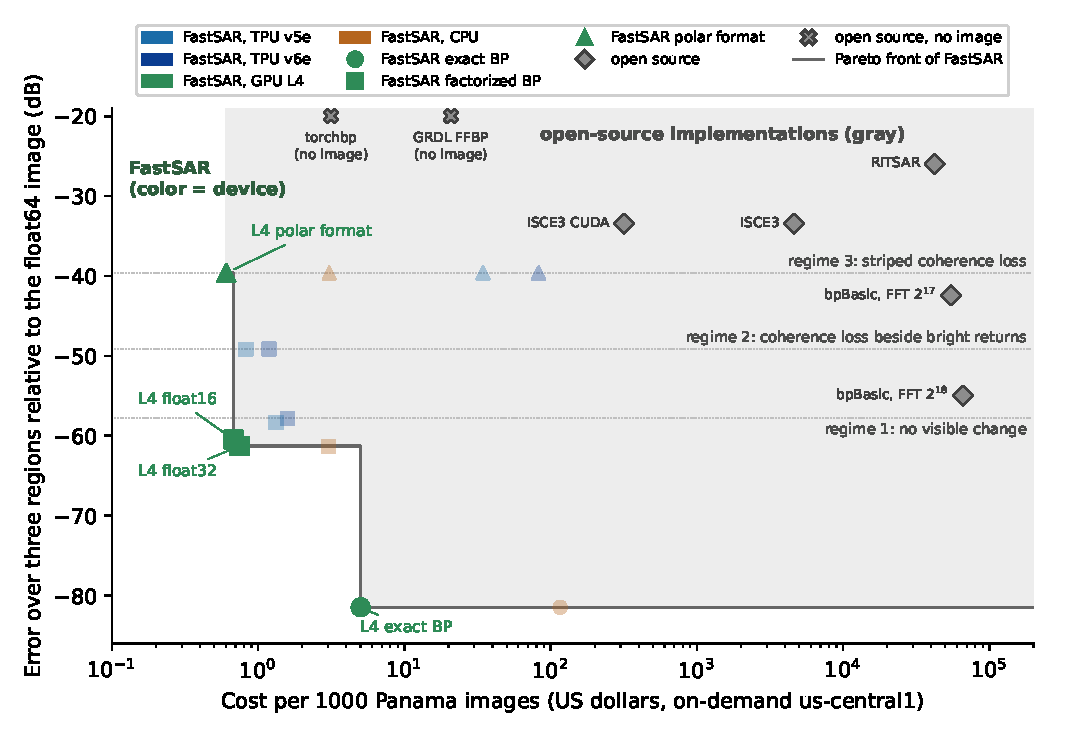
\includegraphics[width=0.9\textwidth]{fig/teaser.pdf}
\caption{Cost per thousand Panama Canal images against the error over the lock, port and ship regions of Figure~\ref{fig:zoom}, for FastSAR on each device and for the open-source implementations on the same CPU instance type and L4 GPU (gray). The three regions are pooled with weights equal to their reference energy. FastSAR's errors are relative to the 64-times computation of Section~\ref{sec:protocol}, the open-source implementations' relative to the reference; ISCE3 is scored as the mean over its own three patches. Times marked est.\ are estimates (Section~\ref{sec:oss}). The torchbp and GRDL backprojections, which produced no usable image (amplitude correlation with the reference 0.22 or less, Appendix~\ref{app:oss}), are drawn off scale. The line is the Pareto front of the FastSAR configurations on these pooled region errors (the bold rows of Table~\ref{tab:cost} use whole-image errors); those off the front are drawn faded and unlabeled (Table~\ref{tab:cost} identifies each configuration). Each dotted line marks the worst FastSAR configuration of one of the image-quality regimes~1 to~3 of Section~\ref{sec:quality}.}
\label{fig:teaser}
\end{figure}

\section{Related work}
\label{sec:prior}

Backprojection on parallel hardware has been reported since 2009 on FPGAs~\cite{cordes2009}, many-core CPUs~\cite{park2012} and GPUs. On GPUs, single-GPU CUDA implementations~\cite{fasih2010}, gigapixel formation on GPU clusters~\cite{benson2012}, nonuniform FFT interpolation~\cite{capozzoli2013} and float16 arithmetic~\cite{xu2022} have been described. Fast factorized backprojection follows the quadtree of McCorkle and Rofheart~\cite{mccorkle1996} and the formulation of Ulander, Hellsten and Stenstr\"om~\cite{ulander2003}; it has been applied to nonlinear tracks~\cite{frey2009} and to circular SAR on GPUs~\cite{ponce2011}. Polar format is described in~\cite{carrara1995,jakowatz1996}; Jakowatz and Doren compared it with backprojection~\cite{jakowatz2006}, and Doerry~\cite{doerry2007} and Gorham and Rigling~\cite{gorham2016} derived its scene-size limit. 

Among open-source implementations, RITSAR~\cite{ritsar}, GRDL~\cite{grdl} and ISCE3~\cite{isce3} run on the CPU, as does the AFRL toolbox~\cite{gorham2010}, distributed by the National Geospatial-Intelligence Agency, with the backprojection \texttt{bpBasic} and the polar format \texttt{pfa\_mem}. On the GPU there are torchbp~\cite{torchbp} and ISCE3's CUDA version. Outside machine learning the TPU~\cite{jouppi2017,jouppi2023} has been used for Fourier transforms~\cite{lu2020,lu2021} and linear algebra~\cite{lewis2022}. No published TPU implementation of SAR image formation, and no comparison of the open-source implementations on matched hardware against a common float64 reference, was found.

\section{FastSAR}
\label{sec:fastsar}

FastSAR takes a phase history, the antenna positions and an output grid and returns a complex image. The CPU, CUDA and TPU backends share the host-side float64 geometry and the factorization plan, including its decimation filters, and stripmap and sliding-spotlight collections are formed as mosaics of factorized patches. Its three algorithms are described in Appendix~\ref{app:algorithms}: factorized backprojection (factorized BP in the tables) follows~\cite{mccorkle1996,ulander2003}. Exact backprojection (exact BP)~\cite{gorham2010} reads range profiles, oversampled 8 times by default from release 0.1.1 (4 times in 0.1.0), with cubic interpolation. Polar format~\cite{carrara1995,jakowatz1996} ends with a resampling that removes its planar-wavefront displacement (Appendix~\ref{app:pfa}).

The factorized kernels are written in C++ with OpenMP for the CPU, in CUDA for NVIDIA GPUs and in Pallas, JAX's kernel language, for TPUs (the fused kernels of the tables; Appendix~\ref{app:kernels}). They replaced a pure JAX implementation (the JAX program), which remains in the library and is timed on the CPU in the release records. In device time the kernels formed the float32-class Panama image @@kgain.v6e.3@@, @@kgain.v5e.3@@ and @@kgain.l4.32@@ times faster than the JAX program on the v6e, v5e and L4. On the CPU the released C++ kernels form it @@kgain.cpu.32@@ times faster than the JAX program (Table~\ref{tab:kernels}). 

The precision options are float32 or float16 throughout (float16 data and tensor-core operands, float32 accumulation) on the GPU and three-pass or single-pass bfloat16 products on the TPU (Appendix~\ref{app:formats}). Exact backprojection has no TPU kernel; on a TPU it runs in pure JAX, at about @@tpuex.v5e.h@@ and @@tpuex.v6e.h@@~h per Panama image on the v5e and v6e (Appendix~\ref{app:tpu}).

\section{Data and protocol}
\label{sec:protocol}

Three spotlight collections from Umbra's open data catalog~\cite{umbra2023} are used throughout (Table~\ref{tab:scenes}, Figure~\ref{fig:scenes}): the Pacific entrance of the Panama Canal (2023-07-18), central Melbourne (2023-02-08) and farmland near Johnston, Iowa (2023-10-20). Each was processed from the Compensated Phase History Data (CPHD) file as delivered onto the vendor's image grid, on the four devices of Table~\ref{tab:platforms}: c4d-highmem-16 instances with 8~cores and 16~vCPUs (the CPU instance), an NVIDIA L4, and TPU v5e and v6e.

The four Panama regions of Figure~\ref{fig:zoom} were identified against Sentinel-2 imagery (Appendix~\ref{app:truth}); the lock, port and ship regions, the three scored regions, are used for the comparison with open-source implementations. Five Capella collections~\cite{capella2023} extend the evaluation to a second vendor and to other modes (Section~\ref{sec:general}): two spotlights (2024-10-04 and 2025-03-03), a sliding spotlight (2022-09-30; Capella's mode SS) and two stripmaps (2021-11-12 and 2025-12-08).

% BEGIN GEN scenes
% END GEN scenes

\begin{figure}[p]
\centering
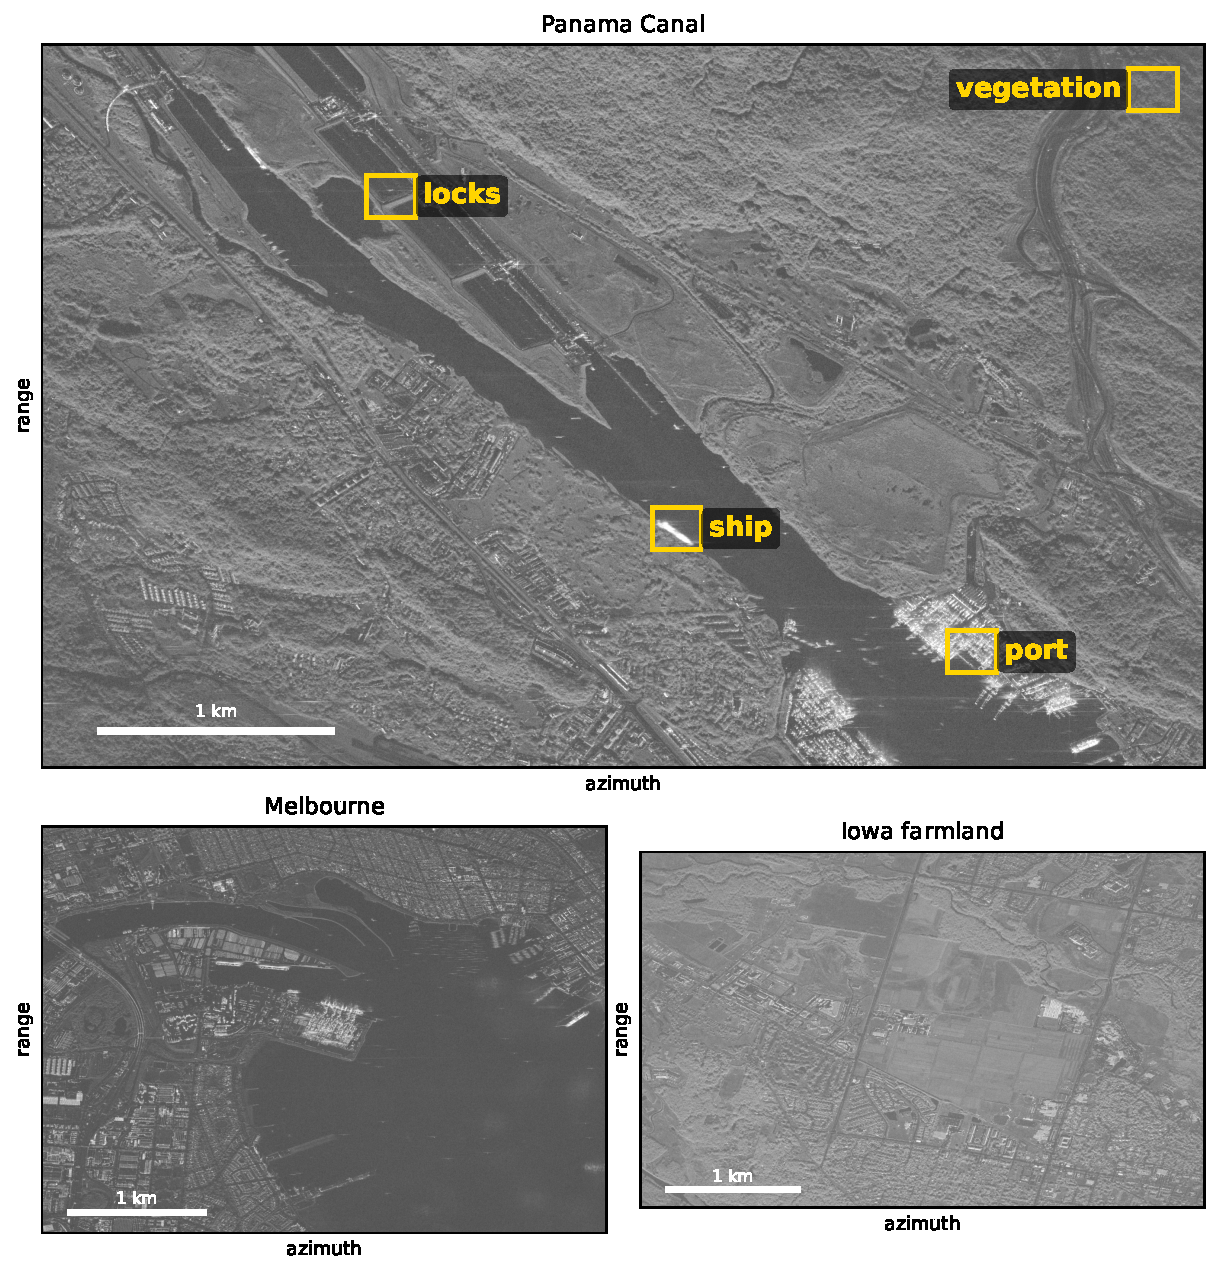
\includegraphics[width=0.92\textwidth]{fig/scenes.pdf}
\caption{The three collections as formed by the reference (Section~\ref{sec:protocol}), downsampled for display (amplitude in decibels over a 45~dB range, azimuth horizontal, range vertical, 1~km bar). The yellow boxes on the Panama Canal image are the four 512 by 512~pixel regions of Figure~\ref{fig:zoom}.}
\label{fig:scenes}
\end{figure}



% BEGIN GEN platforms
% END GEN platforms

Images are compared, after one fitted gain, with the reference, a float64 exact backprojection of the same collection with range profiles oversampled 16 times. Once the vendor's image is resampled through the planar-wavefront displacement model, the reference agrees with it in position to within 0.25~pixel root-mean-square (Appendix~\ref{app:sicd}). The error is the energy of the difference relative to that of the reference, in dB, over the whole image unless stated otherwise (Appendix~\ref{app:protocol} defines the other statistics). The reference is converged to about @@truth.ref.worst@@~dB, so the region errors of FastSAR in Table~\ref{tab:oss} and Figure~\ref{fig:teaser} are measured against a second float64 computation with profiles oversampled 64 times, the 64-times computation (Appendix~\ref{app:protocol}).

Time is the wall-clock time to form one image on a warm device, from the phase history in host memory to the image in host memory, transfers and per-collection host work included, compilation and disk reads excluded. The shorter of two warm calls is reported; it agrees with the time per image of a back-to-back loop within @@proto.loop.agree@@\% on the CPU and the L4, so differences below @@proto.loop.agree@@\% between rows are not resolved. Cost per image is the hourly price divided by the loop's throughput or, where no loop was run, the price multiplied by the time.

Float32-class accuracy means float32 arithmetic on the CPU and L4 and three-pass products on the TPUs. Each configuration is the library's default for its backend and precision option, through the public interface of release 0.1.0 or of a release candidate; Appendix~\ref{app:protocol} states the differences, the loop mechanics and the tuning status of each algorithm.

\section{Results}
\label{sec:results}

\subsection{Comparison with open-source implementations}
\label{sec:oss}

Of the open-source backprojections evaluated here, ISCE3 is the fastest that produced an image. It would need an estimated 4.8~h for the Panama image on the CPU and 27~min on the L4, against @@t.panama.cpu-c4d16.ffbp.fp32_cpp.s@@~s and @@t.panama.gpu-l4.ffbp.fp32_cuda.s@@~s for FastSAR's factorized backprojection (Table~\ref{tab:oss}). After removal of a fitted linear phase ramp, ISCE3 reaches $-54.9$~dB on the CPU at the scene center and $-31.5$ to $-31.9$~dB off center (Appendix~\ref{app:oss}). 

The lowest open-source error on the three scored regions is that of \texttt{bpBasic} with a $2^{18}$-point FFT. Scored against the reference, it is @@oss.bpb18.margin.locks@@, @@oss.bpb18.margin.port@@ and @@oss.bpb18.margin.ships@@~dB above FastSAR's float32 factorized image on the CPU in the lock, port and ship regions (Table~\ref{tab:oss} lists FastSAR against the 64-times computation, so its FastSAR rows are lower than this comparison by the reference's own error).



The two open-source polar-format implementations, \texttt{pfa\_mem} (44.5~s) and GRDL's polar format (24.5~s), leave the planar-wavefront displacement uncorrected. Their log-amplitude correlations with the reference, 0.80 to 0.89 and 0.78 to 0.93, are below the @@osspfa.fastsar.logamp@@ of FastSAR's polar format (Table~\ref{tab:osspfa}).

FastSAR's exact backprojection forms the full image in @@exact.cpu.dur@@ on the CPU and @@exact.l4.dur@@ on the L4, @@exact.isce3.cpu.ratio@@ and @@exact.isce3.l4.ratio@@ times faster than the ISCE3 estimates, with region errors of @@truth.l4exact.range@@~dB. Scaling by pixel count overpredicted the full-image time of FastSAR's exact backprojection on the CPU by a factor of @@exact.cpu.est.factor@@ (@@exact.cpu.est.dur@@ predicted, @@exact.cpu.dur@@ measured), so the open-source estimates and the speed ratios derived from them should be read as upper bounds.

\begin{table}[tbp]
\centering
\caption{Error against the reference and time per full image on the Umbra Panama collection. Errors (dB, Section~\ref{sec:protocol}) are the range over the lock, port and ship regions of Figure~\ref{fig:zoom}, worst to best. ISCE3 was scored instead on three 256 by 256~pixel patches of its own grid (the scene center and two off-center positions), after removal of a linear phase ramp fitted to each. An error of 0.0~dB means that the difference has the same energy as the reference. FastSAR's errors are measured against the 64-times computation, those of the open-source implementations against the reference (Section~\ref{sec:protocol}). $16\times$, $8\times$ and $2\times$ give the oversampling of the range profiles; FastSAR's exact backprojection interpolates them cubically, the others linearly. Times are measured, except those marked est., which scale the time on the scored regions by the number of pixels (Section~\ref{sec:oss}).}
\label{tab:oss}
\small
\begin{tabular}{llrr}
\toprule
Implementation & Instance & Error (dB) & Time per full image \\
\midrule
RITSAR, as published, $16\times$ & CPU & $-25.3$ to $-27.3$ & 44~h (est.) \\
\texttt{bpBasic}, FFT $2^{17}$ (default) & CPU & $-38.1$ to $-43.2$ & 57~h (est.) \\
\texttt{bpBasic}, FFT $2^{18}$ & CPU & $-52.9$ to $-55.4$ & 69~h (est.) \\
ISCE3 \texttt{backproject} & CPU & $-31.5$ to $-54.9$ & 4.8~h (est.) \\
GRDL, factorized & CPU & no image$^\dagger$ & 77.5~s \\
FastSAR, exact, $8\times$ & CPU & @@truth.cpuexact.range@@ & @@exact.cpu.dur@@ \\
FastSAR, factorized, float32 & CPU & @@truth.cpu32.range@@ & @@t.panama.cpu-c4d16.ffbp.fp32_cpp.s@@~s \\
\midrule
ISCE3 \texttt{backproject}, CUDA & L4 & $-31.5$ to $-52.2$ & 27~min (est.) \\
torchbp, exact, $2\times$ & L4 & no image$^*$ ($0.0$) & 16.0~s \\
torchbp, factorized & L4 & no image$^*$ & out of memory \\
FastSAR, exact, $8\times$ & L4 & @@truth.l4exact.range@@ & @@exact.l4.dur@@ \\
FastSAR, factorized, float32 & L4 & @@truth.l432.range@@ & @@t.panama.gpu-l4.ffbp.fp32_cuda.s@@~s \\
FastSAR, factorized, float16 throughout & L4 & @@truth.l416.range@@ & @@t.panama.gpu-l4.ffbp.f16_cuda.s@@~s \\
\bottomrule
\end{tabular}

\smallskip
\begin{minipage}{0.92\textwidth}\footnotesize
$^*$torchbp evaluates the pixel-to-antenna distance in float32. At the 744~km mid-aperture range of this collection (Table~\ref{tab:scenes} gives the range at the start of the aperture) the float32 spacing is 6~cm, about two wavelengths, so the phase of each pulse is lost. A float64 evaluation of the same formula forms the image. On the three regions alone, where memory suffices, its factorized backprojection returns an empty image for the same reason.\\
$^\dagger$GRDL's factorized backprojection is a stripmap algorithm; its image of this spotlight collection is smeared in cross-range (Appendix~\ref{app:oss}).
\end{minipage}
\end{table}

\subsection{Image quality}
\label{sec:quality}

In addition to the energy ratio, each image is assigned to one of three regimes by its amplitude deviation and its coherence with the reference over 5 by 5~pixel windows (the 5 by 5 coherence below). These local statistics are sensitive to isolated errors that do not change the energy ratio. Regime~1 requires an amplitude deviation below 0.05~dB at the 99th percentile and a coherence above 0.999 at the 0.1 percentile. In regime~2 the coherence falls below 0.999 only beside bright returns, and in regime~3 it falls below 0.99 in stripes (the underlying statistics are in Table~\ref{tab:prec}).

On Panama only single-pass TPU products fall in regime~2 and only polar format in regime~3; the other configurations meet the regime~1 criteria (Figures~\ref{fig:zoom} and~\ref{fig:pixels}, Table~\ref{tab:prec}). The errors of the float32-class images are @@p.gpu-l4.ffbp.fp32_cuda.err@@~dB on the L4, @@p.cpu-c4d16.ffbp.fp32_cpp.err@@~dB on the CPU, and @@p.tpu-v6e.ffbp.fp32_high_pallas2_direct.err@@ and @@p.tpu-v5e.ffbp.fp32_high_pallas2_direct.err@@~dB with three-pass products on the v6e and v5e. The JAX program on the CPU, which like the TPU kernels evaluates the last level from float32 geometry, gives @@p.cpu-c4d16.ffbp.fp32.err@@~dB, which suggests that the float32 last level accounts for most of the TPU images' deficit of up to @@q.tpu.vs.f64geo.db@@~dB.

Relative to the float32-class images, float16 throughout on the L4 adds @@l4.f16.loss@@~dB of error and single-pass products on the TPUs add @@sp.vs.3pass.db@@~dB, increases that match the 11 and 8 significant bits of the two formats (Appendix~\ref{app:formats}). The phase deviation of the single-pass v6e image is @@p.tpu-v6e.ffbp.fp32_fast_pallas2_direct.ph99@@$^\circ$ at the 99th percentile but reaches @@p.tpu-v6e.ffbp.fp32_fast_pallas2_direct.phmax@@$^\circ$ beside bright returns (@@sp.phmax.worst@@$^\circ$ on @@sp.phmax.worst.scene@@); its effect on interferometric products was not evaluated. The polar-format error is @@p.gpu-l4.pfa.fp32_taps_corr.err@@~dB, growing from @@pfa.ring.inner@@~dB in the inner ring to @@pfa.ring.outer@@~dB in the outer ring; the cause of this residual was not identified (Appendix~\ref{app:pfa}).

The error of FastSAR's exact backprojection, with cubic interpolation of profiles oversampled 8 times, is @@truth.l4exact.worst@@ to @@truth.l4exact.best@@~dB in the three scored regions against the 64-times computation, @@truth.margin.lo@@ to @@truth.margin.hi@@~dB below the float32 factorized image. Over the whole image it is @@p.gpu-l4.bp.cubic.err@@~dB against the reference, the reference's limit; Appendix~\ref{app:protocol} gives the 4-times and linear variants.

\begin{figure}[p]
\centering
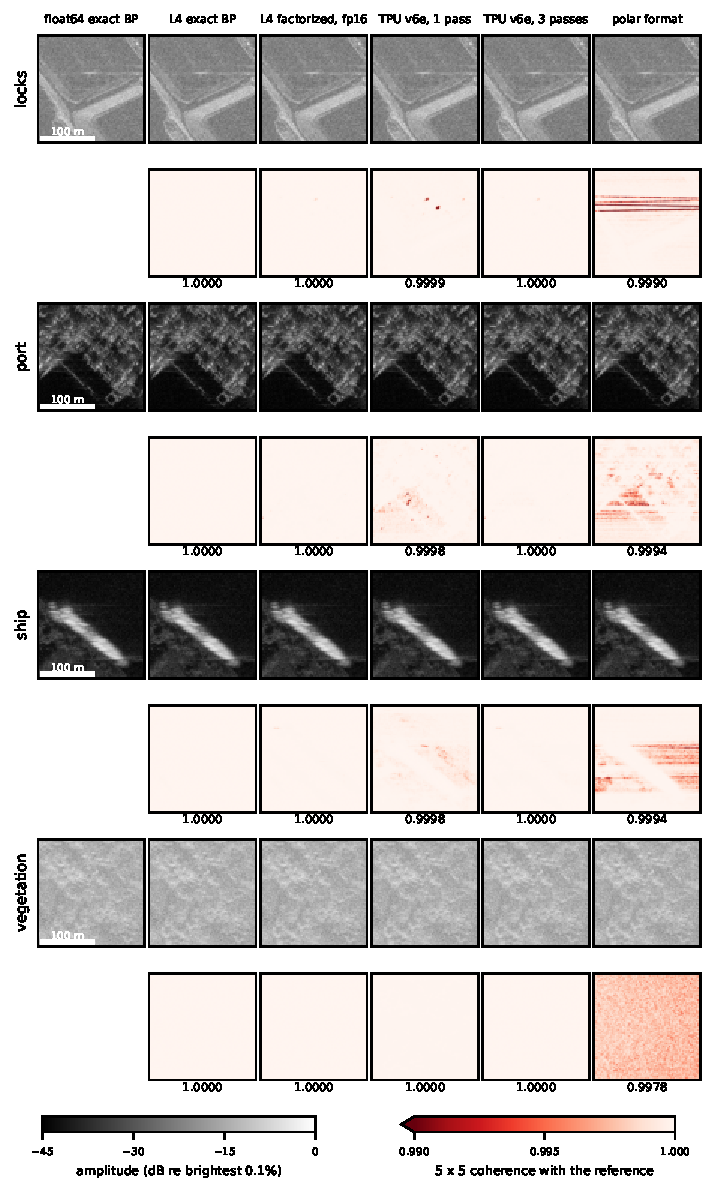
\includegraphics[height=0.80\textheight]{fig/zoom_panama.pdf}
\caption{Panama Canal, four regions of 512 by 512 pixels at full resolution (100~m bar). Top of each pair: amplitude over a 45~dB range for the reference, exact backprojection on the L4 (cubic, $8\times$), factorized backprojection on the L4 in float32 and in float16 throughout, the TPU v6e factorized image with single-pass and three-pass products, and polar format on the L4. Bottom: the 5 by 5 coherence of each image with the reference from 0.99 (red) to 1 (white), with its mean below each panel. The regions are the Cocol\'i Locks, the Port of Balboa, a ship in the channel and vegetated terrain 2.7~km from the scene center; Appendix~\ref{app:truth} locates them.}
\label{fig:zoom}
\end{figure}

\begin{figure}[p]
\centering
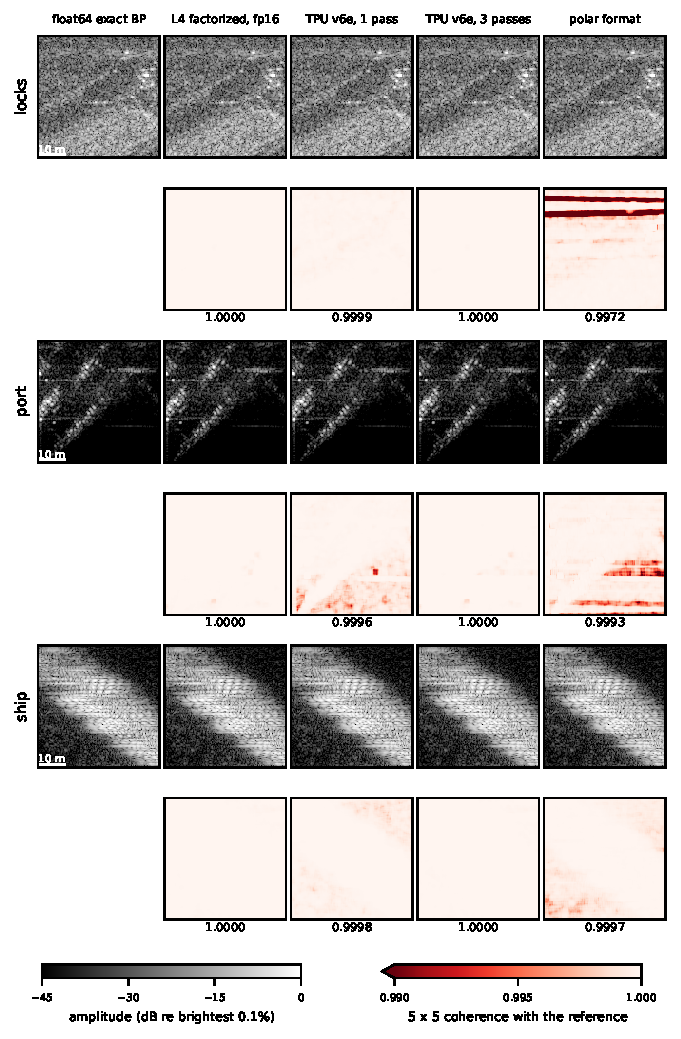
\includegraphics[height=0.74\textheight]{fig/pixels_panama.pdf}
\caption{Panama Canal at pixel scale: 128 by 128~pixel windows (53~m in azimuth by 46~m in slant range, 10~m bar) around the brightest feature of the lock, port and ship regions of Figure~\ref{fig:zoom}, drawn without interpolation (pixel spacing 0.41 by 0.36~m). Columns, scales and coherence maps as in Figure~\ref{fig:zoom}, without the L4 exact backprojection.}
\label{fig:pixels}
\end{figure}

\subsection{Cost per image on CPU, GPU and TPU}
\label{sec:cost}

At float32-class accuracy the cost of a thousand Panama images (Table~\ref{tab:cost}) rises from the L4 (\$@@c.panama.l4.fp32.usd@@) through the v5e (\$@@c.panama.v5e.high.usd@@) and the v6e (\$@@c.panama.v6e.high.usd@@) to the CPU (\$@@c.panama.cpu-c4d16.ffbp.fp32_cpp.usd@@). The order is the same on Melbourne and Iowa, where the L4 costs \$@@c.melbourne.l4.fp32.usd@@ and \$@@c.iowa.l4.fp32.usd@@ and the CPU \$@@c.melbourne.cpu-c4d16.ffbp.fp32_cpp.usd@@ and \$@@c.iowa.cpu-c4d16.ffbp.fp32_cpp.usd@@ (Table~\ref{tab:costother}). The v6e is the fastest device at this accuracy, @@t.panama.tpu-v6e.ffbp.fp32_high_pallas2_direct.s@@~s per image where the L4 takes @@t.panama.gpu-l4.ffbp.fp32_cuda.s@@~s, at @@concl.v6e.price.vs.l4@@ times the L4's hourly price.

Relative to the float32-class configuration on the same device, float16 throughout costs @@l4.f16.saving.pct@@\% less on the L4, a margin only slightly above the @@proto.loop.agree@@\% timing resolution of Section~\ref{sec:protocol}, and single-pass products cost @@sp.saving.v6e.pct@@ and @@sp.saving.v5e.pct@@\% less on the v6e and v5e. Polar format on the L4 costs \$@@c.panama.gpu-l4.pfa.fp32_taps_corr.usd@@ per thousand images. On the TPUs it takes @@pfa.tpu.vs.ffbp.lo@@ to @@pfa.tpu.vs.ffbp.hi@@ times as long as the three-pass factorized configuration, because its resampling steps are scattered gathers, which run on the TPU's vector unit at about $4 \times 10^7$ reads per second (Appendix~\ref{app:tpu}). Exact backprojection on the L4 costs \$@@exact.l4.usd@@ per thousand images, @@exact.cost.l4.ratio@@ times the float32 factorized cost.

% BEGIN GEN cost
% END GEN cost

\subsection{Other collections and modes}
\label{sec:general}

On the Umbra collections of Melbourne and Iowa, the errors of the factorized configurations are within @@other.ffbp.maxdiff@@~dB of the Panama values (supplementary tables, Appendix~\ref{app:stats}). On the five Capella collections (Table~\ref{tab:modes}), FastSAR's worst-region error over the three devices lies between @@modes.err.worst@@ and @@modes.err.best@@~dB.

On the CPU instance, ISCE3's backprojection would take an estimated @@modes.isce3.ratio.min@@ to @@modes.isce3.ratio.max@@ times as long as FastSAR. The two differ in the receive model (Appendix~\ref{app:algorithms}). Against the reference formed with the CPHD positions, ISCE3's worst-region error is @@modes.isce3.cphd.worst@@ to @@modes.isce3.cphd.best@@~dB, @@modes.isce3.cphd.margin.min@@ to @@modes.isce3.cphd.margin.max@@~dB above FastSAR's. Scored against a reference formed with its own receive model, ISCE3's worst-region error is @@modes.isce3.own.lo@@ to @@modes.isce3.own.hi@@~dB below FastSAR's worst error over the three devices on @@modes.isce3.own.which@@.

GRDL's frequency-domain processors, whose slant-plane images were not scored against the reference, were faster than FastSAR on the CPU for both stripmaps and slower for both spotlights. Its range-Doppler processor formed the 2021 stripmap in @@modes.sm2021.grdl.s@@~s, compared with @@modes.sm2021.cpu.s@@~s for FastSAR on the CPU. Among the FastSAR devices, the v6e has the shortest time on all five collections. The L4 costs less per image than the v6e on all collections except the 2025 spotlight; a thousand images of the 2025 stripmap cost \$@@modes.sm2025.cuda.usd@@ on the L4, \$@@modes.sm2025.tpu.usd@@ on the v6e and \$@@modes.sm2025.cpu.usd@@ on the CPU.



% BEGIN GEN modes
% END GEN modes


\section{Conclusions}
\label{sec:concl}

On the Panama collection a commodity GPU, the L4, forms a float32-class spotlight image for \$@@c.panama.l4.fp32.usd@@ per thousand images, and the two TPU generations and the CPU instance cost 1.8 to 4.1 times as much (Table~\ref{tab:cost}). The ordering holds on the Melbourne and Iowa collections and, except for the 2025 spotlight, on the Capella collections. The time margins over the open-source implementations, @@exact.isce3.cpu.ratio@@ to @@oss.ratio.max@@ times, are large compared with the factor of about four by which the pixel-count scaling was found to overpredict a full-image time (Section~\ref{sec:oss}).

The v6e is fastest on every collection but, at @@concl.v6e.price.vs.l4@@ times the L4's hourly price, costs more per image on all but one. On each device the factorized algorithm's stages run within 1.0 to 2.5 times the bounds of their limiting units (Table~\ref{tab:bounds}). The kernel improvements still identified in the profiles are about 12\% on the v6e and 10\% on the L4 (Appendix~\ref{app:kernels}). Gains beyond this would have to come from a change to the factorization plan itself, whose effect on the bounds was not measured.

Exact backprojection is @@truth.margin.lo@@ to @@truth.margin.hi@@~dB more accurate than the factorized algorithm in the scored regions and 6.4 to 38 times slower, on the L4 and the CPU respectively, and it has no efficient form on the TPU. The reduced-precision options change cost and error by less. Float16 throughout saves @@l4.f16.saving.pct@@\% of the L4 cost for @@l4.f16.loss@@~dB of error. Single-pass TPU products save 25 to 38\% of the TPU cost for about 12~dB, with phase errors of up to @@sp.phmax.worst@@$^\circ$ beside bright returns (Section~\ref{sec:quality}). 



Two residuals remain unexplained: the growth of the polar-format error toward the scene edges and the $-31.5$ to $-31.9$~dB floor of ISCE3's off-center Panama patches. On the Capella collections the ISCE3 comparison turns on the receive model adopted for the reference; with its own model ISCE3 has the lower error on @@modes.isce3.own.n@@ of the five. The cost comparison covers on-demand prices on one GPU and two TPU generations, with the L4 on the smallest host offered and the Capella L4 runs on a larger one (Table~\ref{tab:modes}). H100 and TPU7x instances could not be obtained under the project's quota (Appendix~\ref{app:protocol}).

\paragraph{Acknowledgments.} Portions of the code and of this text were drafted with a large language model. The authors designed the experiments, ran and checked the measurements, and are responsible for the content.

\paragraph{Code and data.} FastSAR is available at \url{https://github.com/saulpingerman/FastSAR} and, as release 0.1.0, from the Python Package Index (\texttt{pip install fastsar}). The cloud run scripts, the measurement records behind every table and the source of this paper are at \url{https://github.com/saulpingerman/sar-accel-study}. The radar data are from the Umbra~\cite{umbra2023} and Capella~\cite{capella2023} open data programs and the optical images from Copernicus Sentinel-2~\cite{sentinel2}; none is redistributed, and the scripts fetch them from their public sources.

\begin{thebibliography}{99}
\bibitem{umbra2023} Umbra Lab, Inc., ``Umbra Open Data Program,'' 2023. [Online]. Available: \url{https://umbra.space/open-data}
\bibitem{capella2023} Capella Space, ``Capella Space Synthetic Aperture Radar Open Dataset,'' 2023. [Online]. Available: \url{https://registry.opendata.aws/capella_opendata/}
\bibitem{raney1971} R. K. Raney, ``Synthetic aperture imaging radar and moving targets,'' \emph{IEEE Trans. Aerosp. Electron. Syst.}, vol. AES-7, no. 3, pp. 499--505, 1971.
\bibitem{sentinel2} European Space Agency, ``Copernicus Sentinel-2 Level-2A surface reflectance, tiles S2B\_17PPK\_20230723 and S2A\_17PPK\_20240223,'' contains modified Copernicus Sentinel data 2023 and 2024, accessed October 2026 through the Earth Search STAC catalog. [Online]. Available: \url{https://registry.opendata.aws/sentinel-2-l2a-cogs/}
\bibitem{fasih2010} A. R. Fasih and T. D. R. Hartley, ``GPU-accelerated synthetic aperture radar backprojection in CUDA,'' in \emph{Proc. IEEE Radar Conf.}, Washington, DC, 2010, pp. 1408--1413.
\bibitem{benson2012} T. M. Benson, D. P. Campbell, and D. A. Cook, ``Gigapixel spotlight synthetic aperture radar backprojection using clusters of GPUs and CUDA,'' in \emph{Proc. IEEE Radar Conf.}, 2012, pp. 853--858.
\bibitem{park2012} J. Park, P. T. P. Tang, M. Smelyanskiy, D. Kim, and T. Benson, ``Efficient backprojection-based synthetic aperture radar computation with many-core processors,'' in \emph{Proc. Int. Conf. High Performance Computing, Networking, Storage and Analysis (SC '12)}, Salt Lake City, UT, 2012.
\bibitem{cordes2009} B. Cordes and M. Leeser, ``Parallel backprojection: A case study in high-performance reconfigurable computing,'' \emph{EURASIP J. Embedded Syst.}, vol. 2009, art. 727965, 2009.
\bibitem{capozzoli2013} A. Capozzoli, C. Curcio, and A. Liseno, ``Fast GPU-based interpolation for SAR backprojection,'' \emph{Progress In Electromagnetics Research}, vol. 133, pp. 259--283, 2013.
\bibitem{xu2022} Y. Xu, Z. Zhang, L. Chen, and L. Yang, ``The adaptive streaming SAR back-projection algorithm based on half-precision in GPU,'' \emph{Electronics}, vol. 11, no. 18, art. 2807, 2022.
\bibitem{frey2009} O. Frey, C. Magnard, M. R\"uegg, and E. Meier, ``Focusing of airborne synthetic aperture radar data from highly nonlinear flight tracks,'' \emph{IEEE Trans. Geosci. Remote Sens.}, vol. 47, no. 6, pp. 1844--1858, 2009.
\bibitem{ponce2011} O. Ponce, P. Prats, M. Rodriguez-Cassola, R. Scheiber, and A. Reigber, ``Processing of circular SAR trajectories with fast factorized back-projection,'' in \emph{Proc. IEEE Int. Geosci. Remote Sens. Symp. (IGARSS)}, 2011, pp. 3692--3695.
\bibitem{doerry2007} A. W. Doerry, ``Wavefront curvature limitations and compensation to polar format processing for synthetic aperture radar images,'' Sandia National Laboratories, Albuquerque, NM, Rep. SAND2007-0046, 2007.
\bibitem{gorham2016} L. A. Gorham and B. D. Rigling, ``Scene size limits for polar format algorithm,'' \emph{IEEE Trans. Aerosp. Electron. Syst.}, vol. 52, no. 1, pp. 73--84, 2016.
\bibitem{jakowatz2006} C. V. Jakowatz, Jr. and N. Doren, ``Comparison of polar formatting and back-projection algorithms for spotlight-mode SAR image formation,'' in \emph{Proc. SPIE 6237, Algorithms for Synthetic Aperture Radar Imagery XIII}, 2006, art. 62370H.
\bibitem{jouppi2017} N. P. Jouppi \emph{et al.}, ``In-datacenter performance analysis of a tensor processing unit,'' in \emph{Proc. 44th Annu. Int. Symp. Computer Architecture (ISCA)}, Toronto, ON, 2017, pp. 1--12.
\bibitem{cudaguide} NVIDIA Corporation, ``CUDA C++ Programming Guide,'' Section 5.4.1, Arithmetic instructions, 2025. [Online]. Available: \url{https://docs.nvidia.com/cuda/cuda-c-programming-guide/index.html}
\bibitem{google2024trillium} Google Cloud, ``Introducing Trillium, sixth-generation TPUs,'' May 2024. [Online]. Available: \url{https://cloud.google.com/blog/products/compute/introducing-trillium-6th-gen-tpus}
\bibitem{introl2025} Introl, ``Google TPU architecture: 7 generations explained,'' 2025. [Online]. Available: \url{https://introl.com/blog/google-tpu-architecture-complete-guide-7-generations}
\bibitem{gpuadvisor2025} GPU Advisor, ``TPU v6e (Trillium) specs,'' 2025. [Online]. Available: \url{https://gpuadvisor.com/gpu/tpu-v6e}
\bibitem{tpudocs} Google Cloud, ``Cloud TPU documentation,'' accessed October 2026. [Online]. Available: \url{https://cloud.google.com/tpu/docs}
\bibitem{tpuv6e} Google Cloud, ``TPU v6e,'' Cloud TPU documentation, accessed October 2026. [Online]. Available: \url{https://cloud.google.com/tpu/docs/v6e}
\bibitem{pallasdocs} JAX developers, ``Pallas: a JAX kernel language,'' JAX documentation, accessed October 2026. [Online]. Available: \url{https://docs.jax.dev/en/latest/pallas/index.html}
\bibitem{jouppi2023} N. P. Jouppi \emph{et al.}, ``TPU v4: An optically reconfigurable supercomputer for machine learning with hardware support for embeddings,'' in \emph{Proc. 50th Annu. Int. Symp. Computer Architecture (ISCA)}, Orlando, FL, 2023.
\bibitem{lu2020} T. Lu, Y.-F. Chen, B. Hechtman, T. Wang, and J. Anderson, ``Large-scale discrete Fourier transform on TPUs,'' arXiv:2002.03260, 2020.
\bibitem{lu2021} T. Lu, T. Marin, Y. Zhuo, Y.-F. Chen, and C. Ma, ``Nonuniform fast Fourier transform on TPUs,'' in \emph{Proc. IEEE 18th Int. Symp. Biomedical Imaging (ISBI)}, 2021.
\bibitem{lewis2022} A. G. M. Lewis \emph{et al.}, ``Large-scale distributed linear algebra with tensor processing units,'' \emph{Proc. Natl. Acad. Sci. USA}, vol. 119, no. 33, 2022.
\bibitem{ritsar} D. Macdonald, ``RITSAR: Synthetic aperture radar simulation and processing toolbox for Python,'' 2015. [Online]. Available: \url{https://github.com/dm6718/RITSAR}
\bibitem{isce3} California Institute of Technology, ``ISCE3: InSAR Scientific Computing Environment, version 3,'' releases 0.25.17 and, for the sliding spotlight, 0.25.21, accessed October 2026. [Online]. Available: \url{https://github.com/isce-framework/isce3}
\bibitem{grdl} GEOINT, ``GRDL: GEOINT Rapid Development Library,'' 2026, commit de3338a. [Online]. Available: \url{https://github.com/GEOINT/grdl}
\bibitem{torchbp} H. Forst\'en, ``torchbp: Fast SAR backprojection with PyTorch,'' 2025, commit b371884. [Online]. Available: \url{https://github.com/Ttl/torchbp}
\bibitem{gorham2010} L. A. Gorham and L. J. Moore, ``SAR image formation toolbox for MATLAB,'' in \emph{Proc. SPIE 7699, Algorithms for Synthetic Aperture Radar Imagery XVII}, 2010, p. 769906.
\bibitem{mccorkle1996} J. W. McCorkle and M. Rofheart, ``An order $N^2 \log(N)$ backprojector algorithm for focusing wide-angle wide-bandwidth arbitrary-motion synthetic aperture radar,'' in \emph{Proc. SPIE 2747, Radar Sensor Technology}, 1996, pp. 25--36.
\bibitem{xiao2000} S. Xiao, D. C. Munson, Jr., S. Basu, and Y. Bresler, ``An $N^2 \log N$ back-projection algorithm for SAR image formation,'' in \emph{Conf. Rec. 34th Asilomar Conf. Signals, Systems and Computers}, 2000, pp. 3--7.
\bibitem{ulander2003} L. M. H. Ulander, H. Hellsten, and G. Stenstr\"om, ``Synthetic-aperture radar processing using fast factorized back-projection,'' \emph{IEEE Trans. Aerosp. Electron. Syst.}, vol. 39, no. 3, pp. 760--776, 2003.
\bibitem{carrara1995} W. G. Carrara, R. S. Goodman, and R. M. Majewski, \emph{Spotlight Synthetic Aperture Radar: Signal Processing Algorithms}. Norwood, MA: Artech House, 1995.
\bibitem{jakowatz1996} C. V. Jakowatz, Jr., D. E. Wahl, P. H. Eichel, D. C. Ghiglia, and P. A. Thompson, \emph{Spotlight-Mode Synthetic Aperture Radar: A Signal Processing Approach}. Boston, MA: Kluwer, 1996.
\bibitem{rabiner1969} L. R. Rabiner, R. W. Schafer, and C. M. Rader, ``The chirp z-transform algorithm,'' \emph{IEEE Trans. Audio Electroacoust.}, vol. 17, no. 2, pp. 86--92, 1969.
\bibitem{taylor1955} T. T. Taylor, ``Design of line-source antennas for narrow beamwidth and low side lobes,'' \emph{IRE Trans. Antennas Propag.}, vol. 3, no. 1, pp. 16--28, 1955.
\bibitem{kaiser1974} J. F. Kaiser, ``Nonrecursive digital filter design using the $I_0$-sinh window function,'' in \emph{Proc. IEEE Int. Symp. Circuits and Systems}, 1974, pp. 20--23.
\bibitem{higham2002} N. J. Higham, \emph{Accuracy and Stability of Numerical Algorithms}, 2nd ed. Philadelphia, PA: SIAM, 2002.
\bibitem{wang2019bfloat16} S. Wang and P. Kanwar, ``BFloat16: The secret to high performance on Cloud TPUs,'' Google Cloud Blog, Aug. 2019.
\bibitem{jax2018} J. Bradbury \emph{et al.}, ``JAX: Composable transformations of Python+NumPy programs,'' 2018. [Online]. Available: \url{https://github.com/jax-ml/jax}
\bibitem{lam2015} S. K. Lam, A. Pitrou, and S. Seibert, ``Numba: A LLVM-based Python JIT compiler,'' in \emph{Proc. 2nd Workshop on the LLVM Compiler Infrastructure in HPC}, 2015.
\bibitem{okuta2017} R. Okuta, Y. Unno, D. Nishino, S. Hido, and C. Loomis, ``CuPy: A NumPy-compatible library for NVIDIA GPU calculations,'' in \emph{Proc. Workshop on Machine Learning Systems (LearningSys) at NIPS}, 2017.
\end{thebibliography}

\clearpage
\appendix
\section{Algorithms}
\label{app:algorithms}

The phase history is motion compensated to the scene reference point. For pulse $p$ with antenna position $\mathbf{a}_p$ and frequency sample $f_k$,
\begin{equation}
S_{p,k} = \sum_n \sigma_n \exp\!\left(-j \frac{4\pi f_k}{c}\, \Delta R_p(\mathbf{x}_n)\right),
\qquad
\Delta R_p(\mathbf{x}) = \lVert \mathbf{x} - \mathbf{a}_p \rVert - \lVert \mathbf{a}_p \rVert ,
\label{eq:signal}
\end{equation}
where $\sigma_n$ and $\mathbf{x}_n$ are the complex amplitude and position of scatterer $n$ and $c$ is the speed of light.

The CPHD files give the transmit and receive positions per pulse; their midpoint was used as $\mathbf{a}_p$ (ISCE3~\cite{isce3} instead places the receiver at the transmit position advanced by the velocity times the delay, the receive model of Section~\ref{sec:general}). They also give the start frequency and sample spacing per pulse; the mean values were used, which differ from the per-pulse values by at most @@data.griddrift@@ of a sample spacing.

A Taylor weighting ($\bar{n}=4$, $-35$~dB sidelobes)~\cite{taylor1955} was applied along both axes in every algorithm. The image grid is the vendor's: pixel $(i, j)$ lies at $(i - n_x/2)\,s_x\,\mathbf{e}_1 + (j - n_y/2)\,s_y\,\mathbf{e}_2$ from the reference point. Here $\mathbf{e}_1$ and $\mathbf{e}_2$ are the column and row unit vectors of the vendor's Sensor Independent Complex Data (SICD) product and $s_x$, $s_y$ its sample spacings.

\paragraph{Exact backprojection.} In the reference each pulse is range compressed by a zero-padded inverse FFT with 16 times oversampling. Each pixel is the sum over pulses of the linearly interpolated profile at $\Delta R_p$ times the carrier phase $\exp(j 4\pi f_c \Delta R_p / c)$~\cite{gorham2010}. The range difference is evaluated in the cancellation-free form
\begin{equation}
\Delta R_p(\mathbf{x}) = \frac{q}{1 + \sqrt{1 + q / r_p}}, \qquad q = \frac{\lVert\mathbf{x}\rVert^2}{r_p} - 2\, \hat{\mathbf{u}}_p \cdot \mathbf{x},
\end{equation}
with $r_p = \lVert\mathbf{a}_p\rVert$ and $\hat{\mathbf{u}}_p = \mathbf{a}_p / r_p$. The reference implementation evaluates everything in float64 with Numba~\cite{lam2015} on the CPU.

FastSAR's exact backprojection (\texttt{ExactFormer}, with C++ and CUDA kernels) evaluates the range, the unit vector and the reciprocal range of each tile center in float64 once per pulse. Each pixel's range is then the center's plus a third-order expansion in its offset $\mathbf{d}$ from the center, $\mathbf{d}\cdot\hat{\mathbf{u}} + D/(2r) - (\mathbf{d}\cdot\hat{\mathbf{u}})D/(2r^2)$ with $D = \lVert\mathbf{d}\rVert^2 - (\mathbf{d}\cdot\hat{\mathbf{u}})^2$, evaluated in float32. The tile, 32 by 32 pixels at orbital range, is reduced where the predicted error of the next term would exceed $3\times10^{-4}$~rad. Each pulse is range compressed by a zero-padded FFT, and only the bins its tiles can reach are kept. The profiles are read with cubic Lagrange interpolation (oversampling 8 from release 0.1.1, 4 in release 0.1.0) or linear interpolation (oversampling 8, or 16 on request). On the L4 the Panama image, @@sc.panama.lookups@@~trillion interpolated reads, takes @@t.panama.gpu-l4.bp.cubic.s@@~s, or @@exact.l4.rate@@ billion reads per second.

\paragraph{Factorized backprojection.} The image is divided recursively into tiles, as in the quadtree~\cite{mccorkle1996,xiao2000} and fast factorized~\cite{ulander2003} backprojection algorithms. At each level the phase history of a parent tile is multiplied by $\exp\{j 4\pi f_k (\lVert \mathbf{c} - \mathbf{a}_p \rVert - \lVert \mathbf{c}' - \mathbf{a}_p \rVert)/c\}$ to move its reference point from the parent center $\mathbf{c}'$ to a child center $\mathbf{c}$. The child's signal is then band limited in frequency and in pulse index in proportion to the child's size, and both axes are low-pass filtered and decimated by a Kaiser-windowed sinc~\cite{kaiser1974} with 70~dB design attenuation.

At the last level the range to each pixel is linearized about the tile center and the kernel separates in the two image coordinates. The tile image is then a product of two matrices followed by a per-pixel quadratic phase correction, and no stage requires an indexed read. 

Rectangular images of arbitrary size are handled: the side of each level divides the padded image by factors chosen from 8, 7, 6, 5, 4, 3 and 2. The decimation factors follow from the range and Doppler extents of a child tile. For the Panama image the three levels divide the azimuth side by 8, 8 and 6 and the range side by 8, 7 and 5. The first level decimates the 14,399 samples by 6 and the 15,186 pulses by 4. The final tiles are 32 pixels on a side on all three collections, the default size, which the predicted error supports for each collection geometry.

In the JAX program and the TPU kernels the first two levels compute their phase ramps from float64 geometry on the host and the remaining level from float32 geometry on the device. The CUDA and C++ kernels use float64 geometry at every level. During development a float32 second level was found to add an error that grew with the size of the scene. The ramps themselves are evaluated on the device in float32. The decimation filters are applied as dense matrix products on the TPU, as strided convolutions in the JAX program on the CPU, and as explicit fused multiply-adds in the CUDA and C++ kernels.

\section{Floating-point formats and the arithmetic of each configuration}
\label{app:formats}

Table~\ref{tab:arith} gives the floating-point type of each step of every timed configuration; a development configuration in which the phase ramps were also computed in bfloat16 produced an unusable image, and release 0.1.0 does not offer it.

% BEGIN GEN arith
% END GEN arith

Float16 (IEEE binary16, Table~\ref{tab:formats}) overflows above 65,504, so the phase history is scaled to unit peak before conversion. On the TPU every matrix product is formed from bfloat16~\cite{wang2019bfloat16} operands. A float32 operand is either rounded once (one pass) or split into a bfloat16 head and tail with the cross terms accumulated (three passes); the three-pass product keeps the first 16 significant bits of each operand. A split into three parts (six passes, used by the JAX program) recovers float32 accuracy~\cite{jax2018}. The L4's tensor cores accept float16 operands, which the final stage of float16 throughout uses. The CPU kernels use no reduced-precision arithmetic; the AVX-512 bfloat16 instructions of the processor were not evaluated.

\begin{table}[tbp]
\centering
\caption{Floating-point formats. Significant bits include the implicit bit; the spacing is the distance between adjacent representable values near 1.}
\label{tab:formats}
\begin{tabular}{lrrrl}
\toprule
Format & Bits & Significant bits & Exponent bits & Spacing near 1 \\
\midrule
float64 & 64 & 53 & 11 & $2.2 \times 10^{-16}$ \\
float32 & 32 & 24 & 8 & $1.2 \times 10^{-7}$ \\
float16 (IEEE binary16) & 16 & 11 & 5 & $9.8 \times 10^{-4}$ \\
bfloat16 & 16 & 8 & 8 & $7.8 \times 10^{-3}$ \\
\bottomrule
\end{tabular}
\end{table}

The measured image errors are consistent with the operand resolutions of Table~\ref{tab:formats}. Rounding each operand of the factorized products to bfloat16 adds noise about 48~dB below the operand~\cite{higham2002}. Once the error of the three-pass image is removed, the measured error of the single-pass TPU image agrees to within about 1~dB with the rounding noise of the two operands accumulated through three levels. The L4's float16 operands have 18~dB finer resolution than bfloat16, and their rounding adds @@l4.f16.loss@@~dB to the error of the float32 CUDA build, whose products are all float32.

\section{Exact backprojection on the TPU}
\label{app:tpu}

FastSAR has no TPU kernel for exact backprojection, because the TPU has no fast path for its per-pixel lookup; on a TPU \texttt{ExactFormer} runs in pure JAX (linear interpolation of profiles oversampled 32 times, the accuracy of the cubic default). Timed at the 0.1.1 release candidate \texttt{rel-rc6-20261009} on @@tpuex.v5e.n@@ by @@tpuex.v5e.n@@~pixel grids centered on the Panama lock region, with all pulses, it performed $@@tpuex.v5e.rate@@$ interpolated reads per second on the v5e and $@@tpuex.v6e.rate@@$ on the v6e. At those rates the @@sc.panama.lookups@@~trillion reads of the Panama image take about @@tpuex.v5e.h@@~h (about \$@@tpuex.v5e.usd@@ per image at the instance price) and @@tpuex.v6e.h@@~h (about \$@@tpuex.v6e.usd@@), compared with @@exact.l4.dur@@ on the L4. The grids agreed with the reference to @@tpuex.v5e.err@@ and @@tpuex.v6e.err@@~dB. On a 256 by 256 grid the same program ran at $2.7 \times 10^{7}$ reads per second on the v6e; the slower of the two measurements is used above, and the @@tpuex.v6e.h@@~h figure is therefore an upper estimate.

A TPU core has one or more matrix units, which multiply dense bfloat16 tiles at the chip's rated rate, and a vector unit. In microbenchmarks, data-dependent one-dimensional gathers on the vector unit ran at about $10^8$ reads per second and the scattered two-dimensional gathers of the polar-format resampling at about $4 \times 10^7$ (Appendix~\ref{app:pfa}). Both rates are two orders of magnitude below the matrix units' rate per element.

Google's Cloud TPU documentation~\cite{tpudocs} describes no texture or cache path for scattered reads. The sparse cores of the v6e, intended for embedding lookups, are documented near $10^9$ rows per second per chip~\cite{tpuv6e}, which would still need about 30~min for the Panama image. A one-hot matrix product would move the lookup onto the matrix units, but its matrix has one nonzero in several thousand entries, and the dense product would exceed the work of the factorized algorithm by a comparable factor. The closest published work computes FFTs and nonuniform FFTs, the latter for MRI reconstruction, as matrix products on the TPU~\cite{lu2020,lu2021}.

\section{Kernels for the factorized algorithm}
\label{app:kernels}

% BEGIN GEN kernels
% END GEN kernels

% BEGIN GEN bounds
% END GEN bounds

The factorized rows of Table~\ref{tab:cost} are formed by kernels written for each device after a stage-by-stage profile of the code that XLA, JAX's compiler, generated from the JAX program. On the device, the JAX program took @@kbase.v6e.3.s@@, @@kbase.v5e.3.s@@ and @@kbase.l4.32.s@@~s for the float32-class Panama image on the v6e, v5e and L4, and the last development builds @@knew.v6e.3.s@@, @@knew.v5e.3.s@@ and @@knew.l4.32.s@@~s (the L4 figure is the seventh session's float32 build; its float16-storage build took 2.9~s). On the CPU release 0.1.0 forms the image in @@kbase.cpu.32.s@@~s with the JAX program and @@knew.cpu.32.s@@~s with the C++ kernels. The float32 images of the CUDA and C++ kernels are closer to the reference than that of the JAX program, a difference consistent with their float64 geometry at every level.

In the terms of Appendix~\ref{app:algorithms}, a level splits each parent tile's phase history into those of its children, the tiles of the next level. Level 0 splits the whole collection into the first-level tiles; levels 1 and 2, which run inside one first-level tile per device call, are called the tile levels below. In the JAX program and the TPU kernels only level 2 takes its geometry from the device; the CUDA and C++ kernels compute it in float64 on the host. The plan and filters are the same in every build, and each build's image was checked against the dense image at the same precision on a simulated scene before it was timed. In Table~\ref{tab:kernels}, 16-bit means single-pass products on the TPUs and, on the L4, the float16 variant of each build that the caption lists; float32-class means float32 on the L4 and the CPU and three-pass products on the TPUs.

\paragraph{Diagnosis.} In development, on the v6e, one first-level tile of the Panama image took 51~ms in the JAX program with single-pass products: 8.3~ms in level 0, 13.3 in level 1, 7.9 in level 2 and 21.4 in the final stage. The three levels are bound by memory traffic. XLA writes the rotated phase history of every child (24~bytes per sample, read back by the decimation product) at about 580~GB/s, a third of the v6e's nominal 1,640~GB/s~\cite{google2024trillium} (1,391~GB/s measured, below). The children of the three levels total 63 billion samples per image.

The final stage materializes the two ramp matrices of every 32 by 32 tile ($2T$ by $P_f Q_f$ each, with $T$, $P_f$ and $Q_f$ the tile side and the pulses and frequency samples per tile, defined below) through five or six element-wise passes before the one product that uses them. Its direct form evaluates 400,000 sines and cosines per tile. The same distribution of time is found on the L4, at the lower bandwidth of its convolution path.

\paragraph{TPU kernels (Pallas).} Two Pallas kernels replace the XLA stages. The level kernel takes a block of pulses and a window of columns of a parent into the core's vector memory and applies the phase ramps of up to eight children in turn. Each ramp is the product of a coarse table, one angle per 128-column chunk, and a fine table, one angle per column within the chunk. Both are precomputed once per pulse and child by XLA, and the kernel evaluates no sines. The Pallas documentation~\cite{pallasdocs} lists sines among its most expensive operations, and an earlier build that evaluated the coarse table in the kernel spent a third of its time on them.

The rotated window is multiplied by the banded block of the decimation matrix on the matrix units, in one or three bfloat16 passes. At the two tile levels the pulse-axis decimation is accumulated on the matrix units across the pulse blocks in the same kernel, and neither the rotated window nor the frequency-decimated child reaches high-bandwidth memory. At level 0 the decimated child is too large for vector memory, and the pulse product is a separate dense product.

Children of one parent share each load, and the tile levels batch the parents of a tile into one launch. First-level tiles are formed in groups, and the phase history is read once per group. The development builds of Table~\ref{tab:kernels} used groups of 16; release 0.1.0 uses groups of 4 and also applies the level-0 pulse decimation as a banded product. Where one block of outputs covers a whole row (the tile levels), the window is clipped to the data and read once; at level 0 consecutive output blocks overlap by the filter length.

The final kernel forms the $2T \times 2T$ product of Appendix~\ref{app:algorithms} on the matrix units, where $T = 32$ is the tile side in pixels and $P_f \times Q_f$ the pulses by frequency samples per tile. Both ramps are generated by a complex recurrence along the frequency index $q$. For a pixel offset $d$ along an image axis and the component $u_p$ of the unit vector to the antenna along that axis, the ramp is $\exp(-j 2\pi\, d u_p (a_0 + a_1 q))$. Here $a_0$ and $a_1$ are the cycles per meter at the first frequency sample and per sample step. This equals $X W^q$ with $X = \exp(-j 2\pi d u_p a_0)$ and $W = \exp(-j 2\pi d u_p a_1)$, and one tile needs four tables of sines and cosines of size $T \times P_f$ instead of one sine per sample. 

A first version of this kernel, with one sine per sample, was no faster than the XLA final stage (Table~\ref{tab:kernels}); the recurrence eliminated the sine evaluations, and the stage was no longer bound by the transcendental unit. Other variants tried in development were not kept. Building the level kernel's fine tables in XLA by successive doubling nearly doubled the image time, because each intermediate table of fewer than 128 columns occupies full 128-lane tiles in TPU memory. Evaluating the coarse-table sines over the used lanes alone and padding afterwards cost 4 to 8\%, since XLA holds the table 128 lanes wide either way. Stacking four tiles into one 256 by 256 product in the final stage gained 3\% on the v6e at three-pass precision and nothing otherwise, and lost 2 to 4\% on the v5e, which has 128 by 128 arrays; these differences are within the run-to-run spread of Appendix~\ref{app:protocol}.

\paragraph{Bounds.} The bounds of Table~\ref{tab:bounds} are for the profiled builds of Table~\ref{tab:kernels}, timed on the device; the released library's times from host memory to host memory are those of Table~\ref{tab:cost}.

The unit rates were measured on each device with microbenchmarks in the same framework (\texttt{ubench\_tpu.py} and \texttt{ubench\_gpu.py} in the repository). On the v6e, high-bandwidth memory copies run at 1,391~GB/s. The vector unit executes the level kernel's rotation mix on data resident in vector memory at 117 billion samples per second and a plain copy through vector memory at 155 billion. The rotation therefore runs within a factor of 1.3 of the vector load and store path. XLA evaluates 57 billion sine and cosine pairs per second, and the matrix units reach 457~TFLOP/s on a large bfloat16 product and 42~TFLOP/s at the final stage's 64-row shape.

Against these rates, on the v6e, level 1 runs at the vector unit's rate (ratio 1.0) and level 0 at 1.4 times its vector bound, with the unfused pulse product passing through memory. Level 2 runs at 2.5 times its largest bound but at 0.9 of the sum of the terms that run in sequence: the rotation (0.24~s per image), the sines XLA evaluates for its tables (0.25~s) and the traffic of those tables (0.17~s). The level's rows are 352 samples long, so each child and pulse needs 256 sines for 512 rotated samples. The final stage is 2.2 times its matrix bound; the difference is attributed to the ramp recurrence on the vector unit, which the microbenchmarks did not isolate.

On the v5e the matrix units are about three times slower than the v6e's on a large product, against a vector unit only 12\% slower, and they become the binding unit of levels 0 and 1; each v5e stage lies between its largest bound and the sum of its bounds (1.5 to 2.2 times the former, 0.6 to 0.8 of the latter), so its units overlap only partly.

The largest remaining inefficiency identified within the factorization is the level-2 table generation, which angle-addition tables could reduce by about a factor of eight, about 0.2~s of the 1.7~s device time of the v6e image; the other TPU stages are at most 2.2 times their largest single bound and, where a sum is defined, below the sum of their bounds.

\paragraph{L4 kernels (CUDA).} On the L4 the two kernels are written in CUDA and compiled through CuPy~\cite{okuta2017}. The level kernel loads the window of 32 pulses into shared memory with consecutive threads on consecutive columns, so that global loads are coalesced. It then rotates the window in place for each child, generating the rotation of each thread's samples as a geometric sequence. Each thread then computes two adjacent outputs of one pulse with the 44-tap decimation filter as fused multiply-adds. For this phase consecutive threads are consecutive pulses, so no two threads of a group read the same shared-memory bank. The outputs are staged through shared memory and written row by row. The pulse-axis filter is tiled the same way.

The final kernel builds the two ramp tables of a tile in shared memory by the same recurrence, and each thread accumulates a 4 by 2 block of pixels. In the float16 tensor-core builds the tables are converted to float16 and the $2T \times 2T$ product runs on the tensor cores with float32 accumulation. A Triton version of the level kernel through Pallas, with the 16-column windows its shared-memory limit allows, gained 1 to 4\% with float16 products and was slower in float32 (development device timings, within the run-to-run spread of Appendix~\ref{app:protocol}); the library uses the CUDA builds.

Seven CUDA builds were made and five profiled (Table~\ref{tab:kernels}; the profiles are in the repository). The profile of an early build placed 1.5~s per image in the level kernel, 1.3 in the final stage and 0.5 in the pulse filter. A pulse-major thread mapping removed the bank conflicts from the filter reads but scattered that kernel's global loads and stores, and its time doubled. The following three builds added coalesced loads through shared memory, the geometric-sequence rotation and staged stores, and brought the kernel to 1.9, 1.7 and 1.4~s. The float32 final stage appeared bound by the latency of its table-building recurrence and by one shared-memory word per fused multiply-add; with a 4 by 2 block per thread and interleaved complex tables it fell from 1.3 to 1.0~s. The tensor-core version was 0.43~s faster per image on the device than the float32 one in the sixth build. The seventh build stores the phase history, every intermediate and the final-stage operands in float16 and accumulates in float32 inside the filters, which halves the memory traffic that bounds the level kernel and the pulse filter. It is the float16 configuration of Table~\ref{tab:cost}; release 0.1.0 forms the image with it in @@t.panama.gpu-l4.ffbp.f16_cuda.s@@~s, against @@t.panama.gpu-l4.ffbp.fp32_cuda.s@@~s for the float32 build, with @@l4.f16.loss@@~dB more error.

The L4's measured rates are a memory copy at 246~GB/s, the level kernel's inner mix on resident shared memory at 20.2 billion filter outputs per second, the final kernel's inner mix at 6.1 trillion fused multiply-adds per second (41\% of the chip's peak), and coalesced stores at 252~GB/s, compared with 69~GB/s for strided stores.

Against these, the pulse filter runs at its memory bound and the level kernel at 1.1 times the sum of its arithmetic and memory bounds (1.9 times their maximum; the two overlap only partly at two blocks per multiprocessor). The float32 final stage runs at 2.2 times the bound of its inner mix; the profile places the excess in the table building.

The remaining structural cost of the float32 build is the 172~GB per image that the level kernel writes and the pulse filter reads back; a streaming fusion of the two could remove about half of it, about 0.3~s of the 3.0~s that the profile of the sixth build measures on the device (the three stages of Table~\ref{tab:bounds} account for 2.8~s of it; the development session's own timing of that build, 3.6~s, includes host work). The float16 build halves that traffic instead. In release 0.1.0 it forms the image @@l4.f16.gain.s@@~s faster than the float32 build (Table~\ref{tab:cost}), less than halving a purely memory-bound stage would give. The level kernel's arithmetic bound is close to its memory bound, and float16 storage leaves the arithmetic bound unchanged, since the L4's CUDA cores issue float16 and float32 fused multiply-adds at the same rate (128 per clock per multiprocessor at compute capability 8.9~\cite{cudaguide}). Further gains from float16 on the L4 would depend on the tensor cores, for which the level filters would have to be rewritten as matrix products, as in the TPU kernel.

\paragraph{CPU kernels (C++).} The level filter, the pulse filter and the final stage were written in C++ with OpenMP for the CPU instance, compiled by GCC 13 for AVX-512 with 512-bit vectors preferred, and called from the Python driver through a shared library. The host side (plan, filters, float64 geometry) is the code used for the other devices.

The design that came closest to the arithmetic bound assigns the children of a parent to vector lanes. A sample of the parent row is a scalar broadcast, its rotation one complex multiply per 16 children with a per-lane phase step, and the filter accumulates eight outputs per child vector in registers, so no strided read occurs. The pulse filter reads each input row once per chunk of 16 output rows. The final stage builds its two tables three pulses at a time, by a geometric recurrence over the pulse index and another over the pixel index (four sines per pulse and table). The tables then stay in the second-level cache while the product consumes them.

Four builds were measured (Table~\ref{tab:kernels}). The first, a polyphase filter vectorized along the output columns, took @@kcpu.1.s@@~s per Panama image; its stride-$D$ gathers cost about 12 instructions per useful multiply-add. The second, with children assigned to vector lanes, took @@kcpu.2.s@@~s. The third build (@@kcpu.3.s@@~s) reused the intermediate buffers, which removed one page fault per 4~KB of fresh allocation inside the parallel regions, and kept the accumulators in registers. The fourth (@@kcpu.4.s@@~s, of which 3.8~s was the final stage) builds and consumes the final-stage tables three pulses at a time. The fourth build is the one released; it ran on 8 threads, one per core, and 16 threads gave the same time.

The instance's measured rates are a memory copy at 49~GB/s, the filter's inner loop at 314 billion fused multiply-adds per second on resident data, and the final product's inner loop at 1.04 trillion fused multiply-adds per second. The last figure is near the 8 cores' float32 peak of two 512-bit fused multiply-adds per core and cycle at the measured clock. Against these, the level kernel runs at 1.2 times its arithmetic bound (0.8 of the sum of arithmetic and memory) and the pulse filter at 1.05 times its memory bound. The final stage runs at 1.4 times its arithmetic bound, with the excess in table building (Table~\ref{tab:bounds}).


\section{Polar format on an orbital aperture}
\label{app:pfa}

FastSAR's polar format consists of three resampling steps and a two-dimensional FFT, each expressed with FFTs, element-wise products or a single matrix product so that the same code runs on all devices. The pulses are first resampled so that the tangent of the look angle in the image plane is uniform in pulse index, which an orbit does not give exactly. This is a 16-tap Kaiser-windowed sinc interpolation along the pulse axis, applied as a sum over 16 gathered rows on every device. A dense @@pfa.P@@ by @@pfa.P@@ matrix product, also implemented, needed more than the v5e's 16~GB with its intermediates. Each pulse is then resampled onto a uniform radial wavenumber grid, and each wavenumber row onto a uniform cross-range grid, by chirp-z transforms~\cite{rabiner1969}. These evaluate the band-limited interpolation on a scaled grid with FFTs and chirps; outputs that would wrap around the band are zeroed.

The frequency samples are weighted by $f_c / f_k$ before resampling. Backprojection's uniform weighting of the samples corresponds to a density of $1/k$ in the wavenumber plane (the polar Jacobian) that the uniform spectral weighting of polar format omits; omitting this weighting worsened the error by about 1.5~dB.

Because the grazing angle changes along the aperture, the radial band of each pulse projected onto the image plane drifts from pulse to pulse. The raster covers the union of the bands and so keeps the full spectral support of backprojection, a trapezoid, rather than the inscribed rectangle. For these collections the inscribed rectangle would keep about half the bandwidth in the ground plane and nearly all of it in the vendor's slant plane. The wavenumber grid spacings are set by the native pixel spacings and FFT sizes of @@pfa.nfx@@ by @@pfa.nfy@@, which include a 300~m guard band on every side of the scene. The range and azimuth profiles are tapered to zero within the guard, because the periodic transforms otherwise wrap echoes from beyond the image into its edges (without the guard the edge error was $-5$~dB in development).

\paragraph{Distortion.} Polar format assumes a planar wavefront, and a scatterer at distance $\rho$ from the scene center is then focused about $\rho^2/2R$ from its position in range. At $R = 744$~km (mid-aperture) this is 4~m at 2.5~km, about 12 pixels. The azimuth displacement is larger and depends on the squint (@@pfa.shift.panama.azm@@~m in azimuth and @@pfa.shift.panama.rgm@@~m in range at the Panama corners). The planar model writes the range history of a scatterer at $\mathbf{p}$ as $-\hat{\mathbf{u}}_p \cdot \mathbf{q} + c$. A least-squares fit of $\mathbf{q}$ and $c$ over the aperture to the exact history $\lVert \mathbf{p} - \mathbf{a}_p \rVert - \lVert \mathbf{a}_p \rVert$ gives the position at which polar format focuses the scatterer, $(q_x, q_y + c)$, since a constant range offset is a range shift.

The fit residual is below 1~mrad of phase everywhere in the three scenes, so the image is displaced without defocus, by up to @@pfa.shift.panama.az@@ pixels in azimuth and @@pfa.shift.panama.rg@@ in range at the Panama corners. Measured target positions agreed with the model to 0.2~pixel, and before the final resampling the 5 by 5 coherence with the reference was 0.42. The mapping is fitted by cubic polynomials over the image (residual below $10^{-4}$~pixel).

\paragraph{Final resampling.} The spectrum is placed in a raster of twice the pixel density and transformed without the carrier terms. The result is interpolated at the apparent positions with a six-tap Lanczos kernel along each axis and multiplied by the carriers evaluated at the apparent positions. No separate phase correction is needed; the quadratic phase of about @@pfa.center.quad@@~rad at 211~m seen in development in a center crop before the resampling is the carrier of the range displacement. The oversampled raster is processed in blocks: the range transform is done once, and the azimuth transform and the resampling proceed in blocks of 512 output range columns. The polar-format figures in this paper are for the resampled image.

\begin{figure}[tbp]
\centering
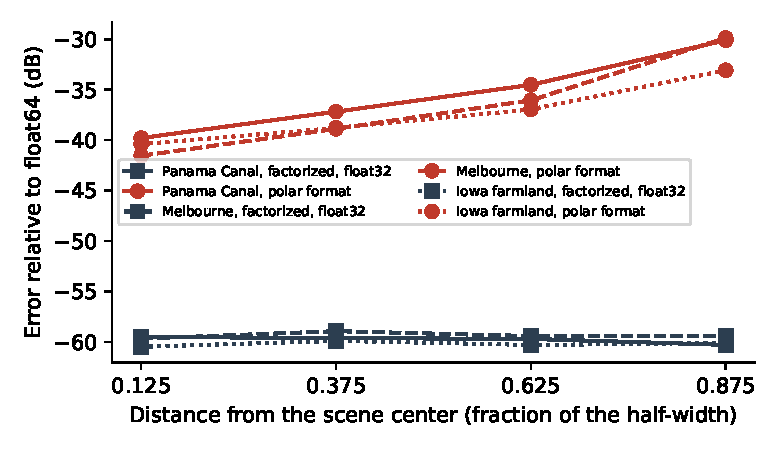
\includegraphics[width=0.72\textwidth]{fig/rings.pdf}
\caption{Error relative to the reference in four concentric rings by distance from the scene center, for the polar-format image and the float32 factorized image on the L4, on the three collections (dB; rings are quarters of the half-width from the scene center outward).}
\label{fig:rings}
\end{figure}

\paragraph{Residual.} After the resampling the error is @@p.gpu-l4.pfa.fp32_taps_corr.err@@~dB on Panama (@@p.melbourne.pfacorr.err@@~dB on Melbourne and @@p.iowa.pfacorr.err@@~dB on Iowa) and the mean 5 by 5 coherence @@p.gpu-l4.pfa.fp32_taps_corr.coh@@. On every collection the residual grows from the inner to the outer ring, by @@pfa.ring.growth.lo@@ to @@pfa.ring.growth.hi@@~dB, from @@pfa.ring.inner@@ to @@pfa.ring.outer@@~dB on Panama, whereas the factorized error shows no dependence on distance from the center (Figure~\ref{fig:rings}). No explanation was found for the residual.

In development, on the full Panama image, the resampling kernel (4, 6 and 8 taps) and the oversampling of the intermediate raster (2 and 3 times) changed the whole-image error by less than 0.6~dB (Table~\ref{tab:pfaedge}). In the outermost ring, where the displacement is 10 to 18~pixels, the change was less than 0.4~dB. Lengthening the pulse interpolator from 16 to 32 or 48 taps, with a narrower Kaiser window, made the error up to 0.9~dB worse. The registration error, measured from the cross-spectrum phase, was 0.001~pixel, and the convergence of the reference is more than 30~dB below the residual. One untested candidate is the Taylor weighting, which backprojection applies per pulse and sample and polar format applies through the resampling onto the rectangular raster; such a difference would grow with distance from the scene center.

\begin{table}[tbp]
\centering
\caption{Panama Canal, polar format on the CPU in development: whole-image error and error by ring (dB) for variations of the final resampling. Rings are the quarters of the half-width from the scene center outward, inner to outer; the selected configuration is the first row.}
\label{tab:pfaedge}
\small
\begin{tabular}{lrrrrr}
\toprule
Variation & Error & Ring 1 & Ring 2 & Ring 3 & Ring 4 \\
\midrule
% BEGIN GEN pfaedge
% END GEN pfaedge
\bottomrule
\end{tabular}
\end{table}

\paragraph{Time.} The final resampling is an indexed read at a computed position, 36 reads per pixel. On Panama the polar-format image takes @@t.panama.gpu-l4.pfa.fp32_taps_corr.s@@~s on the L4 and @@t.panama.cpu-c4d16.pfa.fp32_taps_corr.s@@~s on the CPU, @@pfa.over.ffbp.l4@@ and @@pfa.over.ffbp.cpu@@ times the factorized float32 time on the same device. On the TPUs it takes @@t.panama.tpu-v5e.pfa.fp32_taps_corr.s@@~s (v5e) and @@t.panama.tpu-v6e.pfa.fp32_taps_corr.s@@~s (v6e), @@pfa.tpu.vs.ffbp.lo@@ to @@pfa.tpu.vs.ffbp.hi@@ times the three-pass factorized time, because its final resampling consists of scattered two-dimensional gathers at the rate given in Appendix~\ref{app:tpu}. A separable approximation of the final resampling, expressible as row and column phase ramps, would avoid the scattered gathers. The squinted geometry of these collections is not exactly separable in this way, and the approximation's effect on the TPU's cost was not measured.

\section{Validation against the vendor's image}
\label{app:sicd}

\begin{figure}[tbp]
\centering
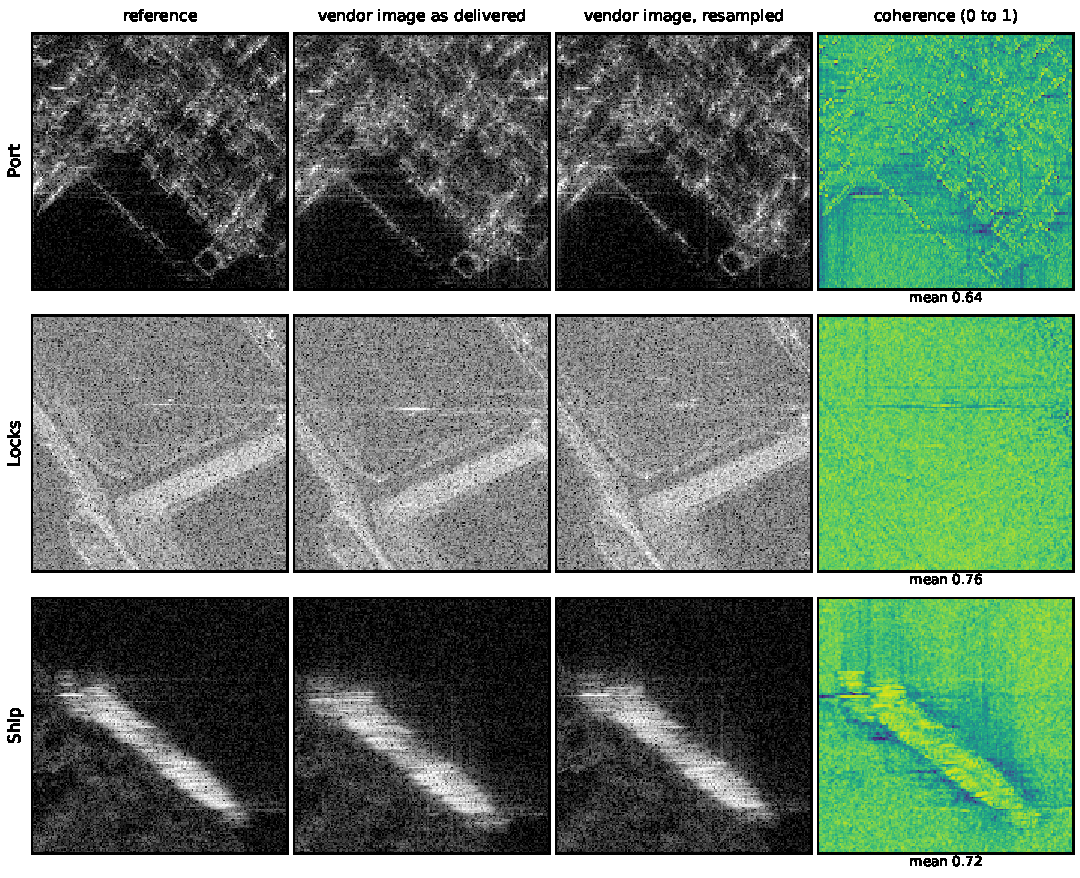
\includegraphics[width=0.94\textwidth]{fig/sicd_panama.pdf}
\caption{The port, lock and ship regions of Figure~\ref{fig:zoom} (rows, 512 by 512 pixels; the row order differs from that figure). Columns: the reference; the vendor image as delivered, on the same pixels; the vendor image after resampling through the planar-wavefront displacement model of Appendix~\ref{app:pfa}; and the 5 by 5 coherence of the resampled vendor image with the reference after local realignment and phase-ramp removal, from 0 to 1, with its mean below each map. Amplitudes are displayed over a 45~dB range.}
\label{fig:sicd}
\end{figure}

Umbra, the vendor, distributes each collection as a complex image in the SICD format, on the pixel grid that the reference adopts; its metadata states that the image was formed from the same phase history by polar format. This allows the reference to be checked against an independent processor. The integer and subpixel offset between the two images (attributed to the vendor's reference-pixel convention) was found from the cross-correlation of block-averaged log amplitude and refined on a central window. The linear phase ramp between them, which reflects the different spectral centering of the two images (@@sicd.panama.ramp.rg@@ cycles per pixel in range on Panama), was found from the peak of the cross-spectrum of the same window and removed.

The vendor image was compared with the reference in 512 by 512 windows centered on a grid with 1024-pixel spacing, keeping the windows with enough contrast for an amplitude cross-correlation (@@sicd.panama.n@@ on Panama). In each window the local offset of the vendor image was measured by amplitude cross-correlation and compared with the displacement that the planar-wavefront model of Appendix~\ref{app:pfa} predicts at the window center. The vendor image was then resampled through the model with a cubic kernel and, after a local realignment and phase-ramp removal in each window, the coherence and the log-amplitude correlation of the two images were computed. As delivered, the vendor image differs from the reference in two respects: it is masked to the parallelogram over which the vendor's processor has full spectral support, and bright points carry cross-shaped sidelobes that the reference's Taylor weighting suppresses.

% BEGIN GEN sicd
% END GEN sicd


The vendor image (Table~\ref{tab:sicd}) is displaced from the reference by a field whose largest value over the Panama windows is @@sicd.panama.meas.az@@~pixels in azimuth and @@sicd.panama.meas.rg@@ in range. The model predicts @@sicd.panama.model.az@@ and @@sicd.panama.model.rg@@ from the collection geometry alone. The root-mean-square difference between measured and predicted displacement over the windows is @@sicd.panama.rms.az@@ and @@sicd.panama.rms.rg@@~pixel on Panama and at most 0.34~pixel on the other two collections, 1 to 4\% of the largest displacement. After the resampling the root-mean-square residual displacement is at most 0.25~pixel (individual windows up to 0.43). The coherence of the two images averages @@sicd.panama.coh@@, @@sicd.melbourne.coh@@ and @@sicd.iowa.coh@@ on Panama, Melbourne and Iowa (@@sicd.panama.wcoh@@, @@sicd.melbourne.wcoh@@ and @@sicd.iowa.wcoh@@ as the median over windows), and their log amplitudes correlate at @@sicd.panama.wlog@@ to @@sicd.iowa.wlog@@ within windows (Figure~\ref{fig:sicd}).

At the brightest isolated points of the lock and port regions (the ship is a moving target and the vegetated region has no isolated point) the impulse-response widths of the two images differ by 1 to 27\%. The vendor's response is wider in azimuth at both points and, in range, narrower at one and 1.3\% wider at the other, which is consistent with a different aperture weighting in the vendor's processor. The SICD metadata does not state whether autofocus was applied, and the vendor's motion compensation is independent of the one used here. Coherence at this level is attributed mainly to the differences between the two processors and is not used as a measure of precision. The vendor image is delivered without a correction for the displacement; the polar-format images of this study remove it in the final resampling (Appendix~\ref{app:pfa}).

The Capella 2021 stripmap and 2024 spotlight of Section~\ref{sec:general} were compared with the vendor's image on the vendor's pixel grid by the same method. The correlation of linear amplitudes is @@modes.vendor.sm2021@@ for the stripmap mosaic (165 patches, 512 by 512~pixel crop) and @@modes.vendor.sp2024@@ for the spotlight formed by exact backprojection (128 by 128 pixels at the scene center); neither figure is comparable with the windowed log-amplitude correlation of Table~\ref{tab:sicd}. In both of these CPHD files the phase sign declared in the metadata is opposite to the sign with which the data focus, and FastSAR's reader reverses it.

\section{Comparison with open-source implementations}
\label{app:oss}

RITSAR~\cite{ritsar} (commit 0e36d2e, ported to Python~3) is a NumPy library. \texttt{bpBasic} is the backprojection of the AFRL toolbox of Gorham and Moore~\cite{gorham2010}, distributed by the National Geospatial-Intelligence Agency (commit 63f0401); it was run in GNU Octave 8.4. ISCE3~\cite{isce3} (0.25.17; 0.25.21 for the Capella sliding spotlight) has C++/OpenMP and CUDA versions, and torchbp~\cite{torchbp} (commit b371884) is a PyTorch extension with CUDA kernels. GRDL~\cite{grdl} (commit de3338a) is a Python library with Numba kernels that reads CPHD files and implements polar format and fast factorized backprojection, run with its default parameters.

All implementations received the Taylor-windowed phase history and antenna positions of the reference (Appendix~\ref{app:algorithms}) in their own input formats and were scored with the error measure of Section~\ref{sec:protocol} on three of the regions of Figure~\ref{fig:zoom}, ISCE3 on 256 by 256~pixel patches of its own radar grid. The whole instance was available to every run; ISCE3 kept about 5.6 of the 16~vCPUs busy. The scripts, records and a longer account of each comparison are in the directory \texttt{results/comparison} of the study repository.

RITSAR's error arises from two indexing defects. Its range axis is built with \texttt{linspace}, so the spacing is too large by one part in $N_{\rm fft}-1$, and its frequency axis is centered on the assumption of an even sample count, which the 14,399 samples of the collection do not satisfy. The error of \texttt{bpBasic} falls by 12 to 15~dB per doubling of its FFT length, as linear interpolation of the range profiles predicts. At $2^{17}$ it stays @@oss.bpb17.vs.lin.lo@@ to @@oss.bpb17.vs.lin.hi@@~dB above FastSAR's exact backprojection with linear interpolation of profiles oversampled 8 times (region errors in the study records). This gap is attributed to \texttt{bpBasic} referencing the phase of its profiles to the lowest frequency of the band.

ISCE3's amplitude correlates with the reference at 0.999 or more; most of its complex difference is a linear phase ramp common to all patches, of the kind that a difference in spectral centering would produce. Once the ramp is removed, the center patch agrees to $-54.9$~dB and the off-center patches retain an unexplained residual of $-31.5$ to $-31.9$~dB.

The torchbp kernels evaluate the distance in float32 (Table~\ref{tab:oss}, footnote); its exact backprojection forms no image, whereas a float64 evaluation of the same formula does. Its factorized backprojection required more than 23~GiB, which exceeds the 22.0~GiB that PyTorch reports as the L4's capacity. GRDL's factorized backprojection, which its documentation describes as a stripmap algorithm, ran on the CPU in 77.5~s. Its image of the spotlight collection is smeared in cross-range, and no orientation of its grid registers to the reference (amplitude correlation 0.22 or less).

The AFRL toolbox also contains a polar format, \texttt{pfa\_mem}, run unmodified in Octave on the same instance (with a compatibility version of \texttt{cross} for mixed row and column inputs), and GRDL's polar format ran on the same instance. Neither image is corrected for the planar-wavefront displacement. Each region was therefore registered and resampled onto the reference pixels before scoring by amplitude statistics and coherence, as for the vendor image of Appendix~\ref{app:sicd} (Table~\ref{tab:osspfa}); part of their coherence loss comes from that resampling.

\begin{table}[tbp]
\centering
\caption{Polar-format implementations on the Panama collection, on the CPU instance: correlation of the log amplitude with the reference and mean coherence in 5 by 5~pixel windows over the three regions, and the time per full image (s).}
\label{tab:osspfa}
\small
\begin{tabular}{lrrr}
\toprule
Implementation & Log-amplitude correlation & Coherence & Time per full image \\
\midrule
AFRL toolbox \texttt{pfa\_mem} (Octave) & 0.80 to 0.89 & 0.76 to 0.88 & 44.5~s \\
GRDL \texttt{PolarFormatAlgorithm} & 0.78 to 0.93 & 0.83 to 0.94 & 24.5~s \\
FastSAR polar format, float32 & @@osspfa.fastsar.logamp@@ & @@osspfa.fastsar.coh@@ & @@t.panama.cpu-c4d16.pfa.fp32_taps_corr.s@@~s \\
\bottomrule
\end{tabular}
\end{table}

\section{Measurement protocol in detail}
\label{app:protocol}

\paragraph{Software and builds.} The software comprised FastSAR release 0.1.0 or the release candidates below, JAX 0.11.2~\cite{jax2018}, CUDA 12 with CuPy 14.2.0~\cite{okuta2017}, and Numba 0.68.0~\cite{lam2015} for the reference. The Umbra records were made at the release-candidate tags \texttt{rel-rc3-20261009} (CPU and TPUs) and \texttt{rel-rc5-20261009} (L4), the Capella records at \texttt{rel-rc2-20261009} (CPU and v6e) and \texttt{rel-rc5-20261009} (L4). At \texttt{rel-rc2} and \texttt{rel-rc3} the library code differs from release 0.1.0 only in the CUDA path and the GPU memory settings, which the CPU and TPU records do not exercise, and at \texttt{rel-rc5} only in one docstring.

The exact backprojection records (Tables~\ref{tab:oss}, \ref{tab:cost} and~\ref{tab:costother}, Figure~\ref{fig:teaser} and Appendix~\ref{app:tpu}) were remade at \texttt{rel-rc6-20261009} (L4, TPUs) and \texttt{rel-rc7-20261009} (CPU). Their library code differs from release 0.1.0 in the default profile oversampling of \texttt{ExactFormer}, 8 instead of 4 times. At \texttt{rel-rc7} it also includes the fixes to reading long collections listed in the changelog of release 0.1.1, which the Umbra records do not exercise. The Umbra records name their commits, and the Capella records' logs do. Every configuration ran in its own process through the public interface and is the fastest of the implementation variants whose errors agreed within 0.1~dB in development.

\paragraph{Time and cost.} For the factorized algorithm the timed interval of Section~\ref{sec:protocol} includes the per-collection host work (the float64 geometry of all three levels for the CUDA and C++ kernels and of the first two for the TPU kernels). Timing followed the two-warm-call rule of Section~\ref{sec:protocol}; the first warm call was up to @@proto.spread.max@@\% slower where one-time work fell on it (90th percentile of the difference @@proto.spread.p90@@\%), and on the CPU and the L4 the reported time agrees with the loop's time per image within @@proto.loop.agree@@\%.

The loop ran until at least four images had been formed and at least 60~s had elapsed, forming images in sequence on the CPU and the L4 and, on the TPUs, staging the next phase history on a worker thread (\texttt{ImageFormer.stage}, as in the mosaics) while the current image forms; on the CPU, exact backprojection and the JAX program were timed without a loop. The factorized kernels were tuned against the bounds of Table~\ref{tab:bounds}; polar format was not tuned, and its costs are upper bounds. The L4 was hosted by a g2-standard-4 instance for FastSAR on the Umbra collections, a g2-standard-8 for the open-source implementations and a g2-standard-32 for the Capella collections. The process's CPU time was recorded during every run.

\paragraph{Power.} The L4's draw was sampled from \texttt{nvidia-smi} twice a second during the timed loops. The TPU virtual machines and the CPU instance expose no power counters; the TPU ranges, derived from third-party design-power figures, and the pro-rata CPU estimate are in Table~\ref{tab:power} and are marked as estimates.

% BEGIN GEN power
% END GEN power


\paragraph{Precision.} The gain fitted per algorithm family is a complex gain for the backprojections and a real one for polar format, whose phase differs from the reference by a smooth screen before the final resampling. Six statistics are computed for each image. The error is the energy of the difference relative to the energy of the reference (dB); this is the figure quoted when a single number is given. The second is the largest single-pixel difference relative to the brightest pixel (dB). The third is the complex coherence between the two images over a 5 by 5 window, reported as the mean, the 0.1 percentile and the minimum. The fourth and fifth are the amplitude ratio and the phase difference over the brighter half of the pixels, reported as the 99th percentile and the maximum. The sixth is the error in four rings by distance from the scene center.

Table~\ref{tab:prec} gives the main statistics of the Panama configurations, and the supplementary tables give all six for every configuration on every collection.

\paragraph{CPU details.} On the CPU the factorized float32 row comes from the C++ kernels of Appendix~\ref{app:kernels} and exact backprojection from its C++ kernel; polar format runs in pure JAX. The reference was formed on a separate n2-highmem-48 instance (48~vCPUs, \$3.14 per hour on demand) in @@ref.panama.s@@~s per Panama image (about \$@@ref.panama.usd1k@@ per thousand images) and is not part of the cost comparison.

\paragraph{Reference convergence and exact backprojection.} The reference's convergence was measured on a 1024 by 1024 crop by forming the same crop at 8, 16 and 32 times. The 8 times image differs from the 32 times image by @@ref.conv8@@~dB and the 16 times image by @@ref.conv16@@~dB. The 16 times reference was adopted because the 8 times convergence error, $-55.5$~dB, lies within the range of the errors under study. On the lock, port and ship regions the same float64 code with profiles oversampled 64 times (the 64-times computation of Section~\ref{sec:protocol}) differs from the reference by @@truth.ref.worst@@ to @@truth.ref.best@@~dB, the reference's own error.

FastSAR's exact backprojection with linear interpolation of 16 times oversampled profiles, the interpolation of the reference, measures @@p.gpu-l4.bp.linear_ov16.err@@~dB against it; the shared interpolation error cancels, and the figure indicates only agreement between the two implementations. With linear interpolation the error is set by the profile oversampling, @@p.gpu-l4.bp.linear.err@@~dB at 8 times. Against the 64-times computation, cubic interpolation at 8 times oversampling, the default of release 0.1.1, gives @@truth.l4exact.worst@@ to @@truth.l4exact.best@@~dB in the three regions, and cubic at 4 times, the default of release 0.1.0, @@truth.cubic4.worst@@ to @@truth.cubic4.best@@~dB. Linear interpolation of oversampled profiles is the scheme of the open-source implementations (Table~\ref{tab:oss} gives each one's oversampling).

On 512 by 512~pixel grids at the same regions, cubic interpolation at 16 times and linear at 64 times are within 0.3~dB of cubic at 8 times, so more oversampling does not lower the error; the float32 arithmetic and the third-order range expansion of the kernel are the likely source of this floor. With linear interpolation at 16 times oversampling the L4 takes @@t.panama.gpu-l4.bp.linear_ov16.s@@~s per image, about \$@@c16.usd@@ per thousand images.

\paragraph{Limitations of the cost comparison.} The improvements still identified in the factorized kernels are about 12\% on the v6e and 10\% on the L4 in the profiled builds, and none was quantified on the CPU, whose stages run at 1.05 to 1.4 times their bounds (Appendix~\ref{app:kernels}). The factorized plan (32-pixel final tiles, three levels, a passband fraction of 0.4 and 70~dB filter attenuation) kept its defaults on every device; a different factorization would change the bounds themselves, by an amount not measured here. TPU7x and H100 instances were outside the project's cloud quota. The cost of the asterisked row of Table~\ref{tab:cost} is computed from the single-image time, not from a loop. The TPU hosts (24 and 44~vCPUs) are larger than the work needs, while the L4's (4~vCPUs) is the smallest offered. Only on-demand prices were used; spot and committed-use prices were not considered.

\section{Ground truth of the Panama regions}
\label{app:truth}

The identity of the Panama regions used in Figure~\ref{fig:zoom} was checked against Copernicus Sentinel-2 imagery~\cite{sentinel2}. Each pixel of the images formed here was located on the ground from the vendor's SICD header. The pixel's position in the slant plane follows from the scene center point and the row and column unit vectors. The ground point is the intersection of the line through it along the slant plane's normal with the WGS84 ellipsoid at the scene height. The image corners so computed agree with the corner coordinates in the SICD header to within 15~m.

The nearest usable Sentinel-2 acquisition is from 2023-07-23, five days later, at 10~m resolution; a dry-season acquisition of 2024-02-23 is shown as well because clouds cover part of the earlier one. The lock chambers, the quays and container yard of the terminal, and the road beside the vegetation region coincide in the two sensors.

The bright target of the ship region, about 180~m long and close to the eastern bank, does not appear in the vendor's geocoded products of six other passes of this repeat-collection site. Four of those passes are three, four, five and seven days after this collection and two are in February 2024. The pass of 2023-07-25 02:30 UTC repeats the geometry of this collection to within $0.3^\circ$ (azimuth $122.4^\circ$ versus $122.1^\circ$, grazing angle $42.6^\circ$ in both, left-looking). This makes an aspect-dependent return from a fixed object unlikely. The other passes span azimuths from $-72^\circ$ to $223^\circ$ and grazing angles from $40^\circ$ to $63^\circ$.

The pass of 2023-07-23 14:47 UTC precedes the Sentinel-2 image of that day by 64~min, and neither shows anything at the position. It is taken to be a ship in the navigation channel; the Sentinel-2 image of 2024-02-23 shows a different ship nearby. The vendor's geocoded product of this collection places the target inside the outlined crop as well.

The ship appears on the eastern bank, inland of the channel, as a consequence of its motion during the aperture. A stationary-scene processor places a target with line-of-sight velocity $v_r$ at the position whose Doppler history matches, displaced along azimuth by about $R v_r / V$ (here about 100~m per m/s), and the along-track velocity defocuses it~\cite{raney1971}. Exact backprojection takes the antenna position of every pulse as data, so a target moving at constant velocity $\mathbf{v}$ is formed exactly by backprojecting with the track shifted by $-\mathbf{v} t$. This both focuses the target and places it at its position at the aperture center.

The ship was assumed to follow the channel axis (bearing $158^\circ$, from the Sentinel-2 water mask) and its speed was swept from $-8$ to $8$~m/s in a tile around it (Figure~\ref{fig:ship}). The sharpness of the tile, the sum of the squared intensities, is single-peaked at $3.0$~m/s (5.8~knots toward the Pacific). At that speed the peak intensity is 10.6~dB above the stationary-scene image and the ship has moved 469~pixels (194~m) along azimuth into the navigation channel; the position of the water was not used in the estimate. A heading $10^\circ$ farther east ($148^\circ$) gives the same speed with an 18\% lower sharpness peak and a compensated position 22~m away. The images compared in Figures~\ref{fig:zoom} and~\ref{fig:pixels} are the stationary-scene images, in which the ship appears at the same displaced position under every algorithm; the motion analysis was used only to identify the target.

\begin{figure}[p]
\centering
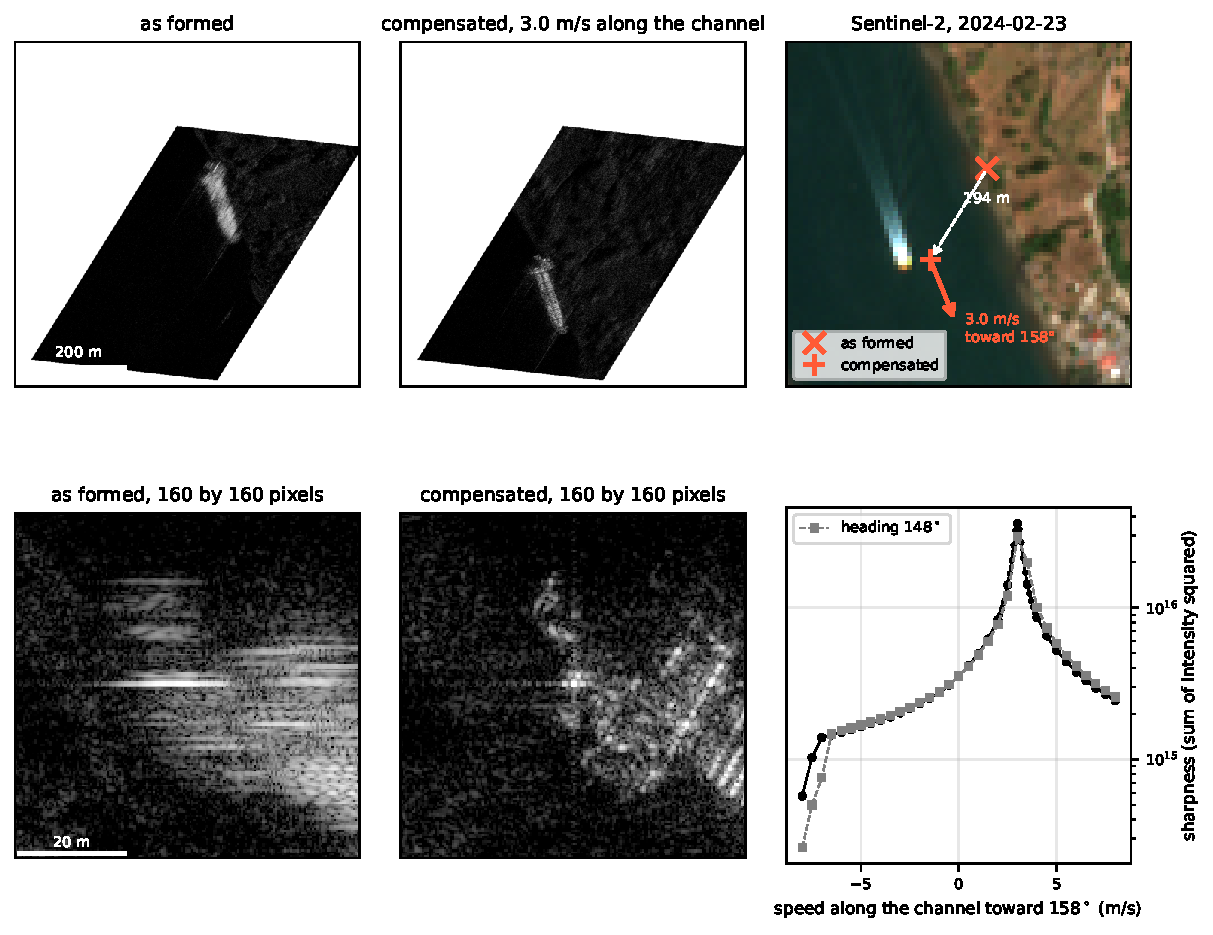
\includegraphics[width=0.96\textwidth]{fig/ship_panama.pdf}
\caption{The ship compensated for its motion. Top: the tile around the ship as formed and after backprojection with the antenna track shifted for a ship moving at 3.0~m/s along the channel, both resampled north up over a 760~m window (200~m bar), and the two positions on the Sentinel-2 image of 2024-02-23, with the 194~m displacement (dashed) and the estimated velocity, 3.0~m/s toward $158^\circ$, drawn at the compensated position. Bottom: 160 by 160~pixel windows around the ship in image coordinates (20~m bar), and the sharpness of the tile against the assumed speed for the channel heading of $158^\circ$ (coarse and fine sweeps) and for $148^\circ$.}
\label{fig:ship}
\end{figure}

\section{Precision and cost tables}
\label{app:stats}

The time and statistics of every configuration on each scene are in the supplementary tables of the study repository (\texttt{paper/supplement\_tables.pdf}); the configuration labels are those of Section~\ref{sec:fastsar}.

% BEGIN GEN costother
% END GEN costother

% BEGIN GEN prec
% END GEN prec


\end{document}
